% Paper II (COLT format). Build: latexmk -pdf discrete   (or pdflatex, bibtex, pdflatex x2)
\documentclass[anon,12pt]{colt2026}
\usepackage{times}
\usepackage{booktabs}
\usepackage{mathtools}
\newtheorem{assumption}{Assumption}
\renewcommand{\theassumption}{\Alph{assumption}}
% Shared math macros (master document and both papers). No theorem environments here.
\providecommand{\R}{\mathbb{R}}
\providecommand{\Z}{\mathbb{Z}}
\providecommand{\E}{\mathbb{E}}
\providecommand{\Prob}{\mathbb{P}}
\providecommand{\nnuc}[1]{\|#1\|_{*}}
\providecommand{\nF}[1]{\|#1\|_{F}}
\providecommand{\inner}[2]{\langle #1, #2\rangle}
\providecommand{\tr}{\operatorname{tr}}
\providecommand{\polar}{\operatorname{polar}}
\providecommand{\Med}{\operatorname{Med}}
\providecommand{\dist}{\operatorname{dist}}
\providecommand{\vol}{\operatorname{vol}}
\providecommand{\rank}{\operatorname{rank}}
\providecommand{\Cov}{\operatorname{Cov}}
\providecommand{\He}{\mathrm{He}}
\providecommand{\cA}{\mathsf{A}}
\providecommand{\cB}{\mathsf{B}}
\providecommand{\ones}{\mathbf{1}}
\providecommand{\st}{\dagger}
\providecommand{\ew}{\varepsilon_w}
\providecommand{\Lw}{L_w}
\providecommand{\SO}{\mathrm{SO}}
\providecommand{\Id}{\mathrm{Id}}
\providecommand{\gs}{g_\ast}
\providecommand{\beff}{b_{\mathrm{eff}}}
\providecommand{\cK}{\mathcal{K}}
\providecommand{\cL}{\mathcal{L}}
\providecommand{\Le}{L_\varepsilon}
\providecommand{\psie}{p}
\providecommand{\argmin}{\operatorname*{arg\,min}}

% Shared statements (bodies only). Each document wraps them in its own theorem environments and labels.
% ---------------------------------------------------------------------------------------------
% Definitions and assumptions
% ---------------------------------------------------------------------------------------------
\newcommand{\StmtClass}{%
Fix constants $0<\lambda\le\Lambda$, $C_\ast\ge1$, $c_\ast\in(0,1]$. For $\varepsilon\in(0,1]$, a random vector $X$ in $E$
belongs to the class $\mathcal X(\varepsilon)$ if there are a covariance $\Sigma$ with
$\lambda\,\Id\preceq\Sigma\preceq\Lambda\,\Id$, a symmetric $3$-tensor $\cK$ with $|\cK|\le C_\ast\varepsilon$, and an even
polynomial $\widehat r$ of degree at most $6$ with $\widehat r(0)=0$ and coefficients bounded by $C_\ast\varepsilon^2$,
such that, with the \emph{comparison transform}
$\widehat\psie(t)=e^{-\inner t{\Sigma t}/2}\big(1+\tfrac16\cK[(it)^{\otimes3}]+\widehat r(t)\big)$ and
$\chi_X(t)=\E e^{i\inner tX}$, $a=c_\ast/\varepsilon$:
\begin{itemize}
\item[\textup{(E1)}] $\int_{t_0+[-a,a]^N}|\chi_X(t)|\,dt\le C_\ast$ for every $t_0\in E$;
\item[\textup{(E2)}] $\int_{[-a,a]^N}|\chi_X(t)-\widehat\psie(t)|\,dt\le C_\ast\varepsilon^3$;
\item[\textup{(E3)}] $\Prob(|X|>u)\le C_\ast e^{-u^2/C_\ast}$ for all $u\ge0$.
\end{itemize}
The \emph{comparison density} is the signed density $\psie$ with $\int e^{i\inner ty}\psie(y)dy=\widehat\psie(t)$; explicitly
$\psie=\varphi_\Sigma\,(1+\frac16\inner{\cK}{\He_3^\Sigma}+r)$ with $r$ an even polynomial. Constants denoted $C,c$ in
statements about $\mathcal X(\varepsilon)$ depend only on $N$, $\nu$, $\lambda,\Lambda,C_\ast,c_\ast$.}

\newcommand{\StmtAssB}{%
$\zeta,\zeta_1,\zeta_2,\dots$ are i.i.d.\ in $E$ with $|\zeta|\le M$ almost surely, $\E\zeta=0$, and covariance
$\Sigma\succeq\lambda\,\Id$, $\lambda>0$; $K_3=\E\zeta^{\otimes3}$. A \emph{weight sequence} is $w=(w_k)_{k\ge1}$ with
$w_k\ge0$, $\sum_kw_k=1$; we set
\[
\rho_p=\sum_kw_k^p,\quad\ \xi_w=\sum_kw_k\zeta_k,\quad\ X_w=\rho_2^{-1/2}\xi_w,\quad\
\ew=\frac{\max_kw_k}{\sqrt{\rho_2}},\quad\ \Lw=\log(e/\ew).
\]
No condition is imposed on the characteristic function of $\zeta$.}

\newcommand{\StmtAssR}{%
There is a closed cone $V\subset E$ such that $o\in C^\infty(E\setminus V)$,
$|D^ko(y)|\le C_k\dist(y,V)^{-k}$ for all $k\ge0$, and
$\vol\{y\in B(0,1):\dist(y,V)\le r\}\le C_Vr^{c}$ for $r\le1$.}

\newcommand{\StmtAssL}{%
$N\ge3$, and there are $\kappa\in(0,1]$ with $2+\kappa<N$ and a constant $C$ such that the Fourier transform of the
finite signed measure $\lambda_\nu=\Delta(\chi\nu)$ satisfies $|\widehat{\lambda_\nu}(t)|\le C(1+|t|)^{-\kappa}$ for all
$t\in E$. Here $\chi$ is a fixed smooth radial cut-off equal to $1$ on $B(0,1)$ and supported in $B(0,2)$.}

\newcommand{\StmtAssN}{%
$\xi_b=\frac1b\sum_{i\le b}\zeta_i$ with $\zeta_i$ i.i.d.\ in $E$, $\E\zeta=0$, $\E|\zeta|^3<\infty$, covariance
$\Sigma\succ0$, third cumulant tensor $K_3=\E\,\zeta^{\otimes3}$, and Cram\'er's condition
$\limsup_{|t|\to\infty}|\E e^{i\inner t\zeta}|<1$.}

% ---------------------------------------------------------------------------------------------
% Paper II statements
% ---------------------------------------------------------------------------------------------
\newcommand{\StmtCodim}{%
Let Assumption~\ref{ass:R} hold with $c\ge2$. There are $\varepsilon_0,C>0$ such that for every
$X\in\mathcal X(\varepsilon)$ with $\varepsilon\le\varepsilon_0$, writing $\Le=\log(e/\varepsilon)$,
\begin{equation}\label{eq:codimX}
\argmin_{x\in E}\ \E\big[\nu(x+X)-\nu(X)\big]\ \subset\ B\big(\hat x,\ C\varepsilon^{\min(c,3)}\Le^{N/2}\big),\qquad
\hat x=-\tfrac16J_\Sigma^{-1}T_\Sigma[\cK],
\end{equation}
In particular, under Assumption~\ref{ass:B}, for every weight sequence with $\ew\le\varepsilon_0$,
\begin{equation}\label{eq:codimw}
\arg\min\psi_{\xi_w}\ \subset\ B\Big(\frac{\rho_3}{\rho_2}\,\gs\,,\ C\sqrt{\rho_2}\;\ew^{\min(c,3)}\,\Lw^{N/2}\Big),
\end{equation}
so that for the mean of $b$ samples
$\Med_\nu(\xi_b)=-\gs/b+O(b^{-3/2}\log^{N/2}b)$ if $c=2$ and $\Med_\nu(\xi_b)=-\gs/b+O(b^{-2}\log^{N/2}b)$ if $c\ge3$.}

\newcommand{\StmtLaplace}{%
Let Assumption~\ref{ass:L} hold and put $q=N/(N-\kappa)\in(1,\frac32]$. There are $\varepsilon_0,C>0$ such that for every
$X\in\mathcal X(\varepsilon)$ with $\varepsilon\le\varepsilon_0$, with $H(x)=\E[\nu(x+X)-\nu(X)]$,
$\Psi(x)=\int(\nu(x+y)-\nu(y))\psie(y)dy$ and $d_\varepsilon=\varepsilon^{q}\Le^{(N+1)/4}$:
\begin{equation}\label{eq:laplaceX}
\sup_{|x|\le2}|H(x)-\Psi(x)|\le Cd_\varepsilon^2,\qquad
\sup_{|x|\le1}\ \sup_{v\in\partial H(x)}|v-\nabla\Psi(x)|\le Cd_\varepsilon,\qquad
\arg\min H\subset B(\hat x,Cd_\varepsilon),
\end{equation}
with $\hat x=-\frac16J_\Sigma^{-1}T_\Sigma[\cK]$. In particular, under Assumption~\ref{ass:B}, for every weight sequence
with $\ew\le\varepsilon_0$,
\begin{equation}\label{eq:laplacew}
\arg\min\psi_{\xi_w}\ \subset\ B\Big(\frac{\rho_3}{\rho_2}\,\gs\,,\ C\sqrt{\rho_2}\;\ew^{q}\,\Lw^{(N+1)/4}\Big),
\end{equation}
so that $\Med_\nu(\xi_b)=-\gs/b+O\big(b^{-1-\frac{\kappa}{2(N-\kappa)}}\log^{\frac{N+1}4}b\big)$ for the mean of $b$ samples.
The middle estimate of \eqref{eq:laplaceX} holds for \emph{every} subgradient, hence for the expectation of every
measurable selection of $\partial\nu(x+X)$, whatever its values on the singular set.}

\newcommand{\StmtNuclear}{%
Let $\nu=\nnuc\cdot$ on $\R^{K\times d}$ with $(K,d)\ne(1,1)$, $N=Kd$, and let Assumption~\ref{ass:B} hold. Then for every
bounded law with nondegenerate covariance, lattice laws included,
\[
\Med_\ast(\xi_b)=-\frac{\gs}b+O\big(b^{-1-\gamma}\log^{N}b\big),\qquad
\gamma=\begin{cases}1&\text{if }|K-d|\ge2,\\[1pt] \tfrac12&\text{if }|K-d|=1,\\[1pt]
\tfrac1{14}&\text{if }K=d=2,\\[1pt] \tfrac1{4K^2-2}&\text{if }K=d\ge3,\end{cases}
\]
and more generally $\arg\min\psi_{\xi_w}\subset B\big(\frac{\rho_3}{\rho_2}\gs,\,C\,(\max_kw_k)\,\ew^{2\gamma}\Lw^{N}\big)$,
uniformly over weight sequences with $\ew\le\varepsilon_0$. For $K=d=1$ the
statement is false (Theorem~\ref{thm:sign}).}

\newcommand{\StmtSign}{%
Let $\zeta$ be a real random variable with $\E\zeta=0$, variance $\sigma^2>0$, $\E|\zeta|^3<\infty$,
$\kappa_3=\E\zeta^3$, and $\gs=\kappa_3/(6\sigma^2)$; let $S_b=\zeta_1+\dots+\zeta_b$ and
$G_b^\st=\arg\min_G\E|G+S_b/b|$.
\begin{enumerate}
\item[\textup{(a)}] If $\zeta$ is not lattice, $b\,G_b^\st\to\gs$ (every selection).
\item[\textup{(b)}] If $\zeta$ is lattice, supported on $a+h\Z$ with maximal span $h$, let $\Lambda_b=-(ba+h\Z)$. For every
$\delta>0$ and $b\ge b_0(\delta)$: $b\,G^\st_b\subset[\gs-\frac h2-\delta,\ \gs+\frac h2+\delta]$, and if a point
$\ell$ of $\Lambda_b$ satisfies $|\ell-\gs|\le\frac h2-\delta$ then $b\,G^\st_b=\{\ell\}$. Consequently:
\begin{enumerate}
\item[\textup{(i)}] if $a/h$ is irrational, the limit points of $b\,G_b^\st$ fill the interval $[\gs-\frac h2,\gs+\frac h2]$;
\item[\textup{(ii)}] if $a/h=p/q$ in lowest terms, then for $b$ in each residue class $j$ modulo $q$ for which $\gs$ is not
a midpoint of $-(\frac{jh}q+h\Z)$, $b\,G_b^\st$ is eventually equal to the point of that coset nearest to $\gs$; there
is no limit if $q\ge2$, and if $q=1$ and $\gs\notin\frac h2+h\Z$ the limit is $h\operatorname{round}(\gs/h)$;
\item[\textup{(iii)}] if $\zeta\in h\Z$ and $|\kappa_3|<3\sigma^2h$, then $G_b^\st=\{0\}$ for all large $b$: sign descent is
exactly unbiased, although $\gs\ne0$ when $\kappa_3\ne0$.
\end{enumerate}
\end{enumerate}
In the lattice case $b\,G_b^\st\to\gs$ only if $a\in h\Z$ and $\gs\in h\Z$.}

\newcommand{\StmtWor}{%
Let $n\ge3$ and $z_1,\dots,z_n\in E$ with $\sum_iz_i=0$, $|z_i|\le M$, $\Sigma_n=\frac1n\sum_iz_iz_i^\top\succeq\lambda\,\Id$,
$K_{3,n}=\frac1n\sum_iz_i^{\otimes3}$, and let $\gs^{(n)}=-\frac16J_{\Sigma_n}^{-1}T_{\Sigma_n}[K_{3,n}]$. Let
$\xi_{n,b}$ be the mean of a uniformly random subset of size $b\in\{1,\dots,n-1\}$, $p=b/n$ and $v=np(1-p)=b(n-b)/n$. Suppose that $\nu$
satisfies Assumption~\ref{ass:R} with $c\ge2$, and put $\gamma=\frac12(\min(c,3)-1)$, or Assumption~\ref{ass:L}, and put
$\gamma=\frac{\kappa}{2(N-\kappa)}$. Then there are $v_0,C$, depending only on $\nu,M,\lambda$, such that whenever
$v\ge v_0$,
\begin{equation}\label{eq:wor}
\sup_{m\in\Med_\nu(\xi_{n,b})}\Big|\,b\,m+\frac{n-2b}{n-2}\,\gs^{(n)}\Big|\le C\,v^{-\gamma}\,\log^{N}(ev).
\end{equation}
In particular the first-order bias of a batch drawn without replacement is that of a batch drawn with replacement
multiplied by $\frac{n-2b}{n-2}$: it vanishes at $b=n/2$ and \emph{changes sign} beyond, for every bounded population
with nondegenerate covariance, lattice populations included, as soon as $b\to\infty$ and $n-b\to\infty$.}

\newcommand{\StmtMomCor}{%
Let $N_\beta=(1-\beta)\sum_{k\ge0}\beta^k\xi_b^{(k)}$ with independent batch means $\xi_b^{(k)}$ of samples satisfying
Assumption~\ref{ass:B}, and let $\beff=b\,\frac{1+\beta+\beta^2}{1-\beta^2}$, $\theta=\frac{1-\beta^2}b$. If $\nu$ satisfies
Assumption~\ref{ass:R} with $c\ge2$ (put $\gamma=\frac12(\min(c,3)-1)$) or Assumption~\ref{ass:L} (put
$\gamma=\frac\kappa{2(N-\kappa)}$), then
\[
\Med_\nu(N_\beta)=-\frac{\gs}{\beff}+O\Big(\frac{\theta^{\gamma}\log^{N}(e/\theta)}{\beff}\Big)
\qquad\text{uniformly in }b\ge1,\ \beta\in[0,1)\text{ with }\theta\le\varepsilon_0^2 .
\]
In particular the first-order law holds at \emph{fixed} batch size, even $b=1$, as $\beta\to1$.}

% ---------------------------------------------------------------------------------------------
% Paper I statements
% ---------------------------------------------------------------------------------------------
\newcommand{\StmtConv}{%
Let $F:E\to\R$ be differentiable, strongly convex, with Lipschitz gradient; let $\nu$ be any norm on $E$ and
$(\xi_t)_{t\ge1}$ i.i.d.\ with $\E|\xi_t|^2<\infty$. From deterministic $W_1,M_0$ run
\[
M_t=\beta M_{t-1}+(1-\beta)\big(\nabla F(W_t)+\xi_t\big),\qquad W_{t+1}=W_t-\eta_tO_t,\qquad O_t\in\partial\nu(M_t),
\]
with $\beta\in[0,1)$ fixed, $O_t$ any measurable function of $(\xi_1,\dots,\xi_t)$ with values in $\partial\nu(M_t)$,
and $\eta_t=\eta_0(t+t_0)^{-\theta}$, $\eta_0,t_0>0$, $\frac12<\theta\le1$. Let
$N_\beta=(1-\beta)\sum_{j\ge0}\beta^j\xi_j$ be the stationary filtered noise. Then, almost surely, $\nabla F(W_t)$ converges
to a (possibly random) point
\[
G_\infty\in\arg\min\psi_{N_\beta}=-\Med_\nu(N_\beta),\qquad\text{and}\qquad W_t\to(\nabla F)^{-1}(G_\infty).
\]
No assumption is made on the law of the noise beyond a second moment: it may be discrete, lattice, or carried by a
proper subspace, and $\partial\nu(M_t)$ may be multivalued with positive probability at every step.}

\newcommand{\StmtCF}{%
Let $\nu$ be the $\ell_1$, the Euclidean or the nuclear norm with its direction map, and let Assumption~\ref{ass:N}
hold. Then for every $\epsilon>0$ there is $b_0$ such that for all $b\ge b_0$
\begin{equation}\label{eq:cf}
\arg\min\psi_{\xi_b}\ \subset\ B\Big(\frac{\gs}b,\frac\epsilon b\Big),\qquad\text{i.e.}\qquad
\Med_\nu(\xi_b)=-\frac{\gs}b+o\Big(\frac1b\Big),\qquad \gs=-\tfrac16\,J_\Sigma^{-1}\,T_\Sigma[K_3].
\end{equation}}

\newcommand{\StmtTwo}{%
Let $K,d\ge2$, $r=\min(K,d)$, $\bar d=\max(K,d)$, $\nu=\nnuc\cdot$ on $\R^{K\times d}$, and let $Z$ be a standard Gaussian
$K\times d$ matrix with singular values $s_1,\dots,s_r$. Put
\begin{equation}\label{eq:q}
m_p=\E\sum_is_i^p,\qquad q_{K,d}=\frac1{m_1}\,\E\sum_{i\ne j}\frac{s_is_j}{s_i+s_j},\qquad c_{K,d}=\frac{m_1}{Kd},
\end{equation}
\begin{equation}\label{eq:a12}
a_1=\frac{3\big[(K-1)(d-1)-2(K+d+1)\,q_{K,d}\big]}{(K-1)(d-1)(K+2)(d+2)},\qquad
a_2=\frac{6\big[(Kd+2)\,q_{K,d}+(K-1)(d-1)\big]}{(K-1)(d-1)(K+2)(d+2)} .
\end{equation}
\begin{enumerate}
\item[\textup{(a)}] \emph{(Reduction.)} For every symmetric $3$-tensor $K_3$ and $\sigma>0$,
$J_{\sigma^2I}=\sigma^{-1}c_{K,d}\,\Id$ and $T_{\sigma^2I}[K_3]=-\sigma^{-3}c_{K,d}\,(a_1\cA[K_3]+a_2\cB[K_3])$, where
$\cA[K_3]_{ij}=\sum_{k,l}K_3^{(ij),(kl),(kl)}$ and $\cB[K_3]_{ij}=\sum_{k,l}K_3^{(kj),(kl),(il)}$. Hence, for a noise law
with covariance $\sigma^2I$ and third cumulant $K_3=\E\zeta^{\otimes3}$,
\begin{equation}\label{eq:two}
\gs=\frac1{6\sigma^2}\Big(a_1\,\E\big[\zeta\nF\zeta^2\big]+a_2\,\E\big[\zeta\zeta^\top\zeta\big]\Big).
\end{equation}
The bias operator $K_3\mapsto\gs$ has rank $Kd$ on a space of dimension $\binom{Kd+2}3$.
\item[\textup{(b)}] \emph{(One number.)} $m_3=(K+d-q_{K,d})\,m_1$; $0<q_{K,d}<\frac{r-1}2$; $a_2>0$.
\item[\textup{(c)}] \emph{(Rank-one and full-rank directions.)}
$a_1+a_2=\dfrac{3(3+2q_{K,d})}{(K+2)(d+2)}$ and $r\,a_1+a_2=\dfrac{3(\bar d-1-2q_{K,d})}{(\bar d-1)(\bar d+2)}>0$.
\item[\textup{(d)}] \emph{(Negative fourth derivative.)} For every $D\ne0$,
$\nabla^4\psi_I(0)[D,D,D,D]=-c_{K,d}\big(a_1\nF D^4+a_2\tr(DD^\top)^2\big)<0$.
\item[\textup{(e)}] \emph{(Proportional limit.)} If $K,d\to\infty$ with $K/d\to\gamma\in(0,1]$, then $q_{K,d}/K\to\kappa(\gamma)$,
$d\,a_2\to6\kappa(\gamma)$ and $d^2a_1\to\frac3\gamma\big(1-2(1+\gamma)\kappa(\gamma)\big)$, where
$\kappa(\gamma)=\big[(1+\gamma)\mu_{1/2}(\gamma)-\mu_{3/2}(\gamma)\big]/\big(\gamma\,\mu_{1/2}(\gamma)\big)$ and
$\mu_s(\gamma)=\int x^s\,d\mathrm{MP}_\gamma(x)$ are the moments of the Marchenko--Pastur law; $\kappa(1)=\frac25$.
\end{enumerate}
For $K=1$ the two contractions coincide and $\gs=\frac{3}{d+2}\cdot\frac{\E[\zeta|\zeta|^2]}{6\sigma^2}$.}

\newcommand{\StmtAone}{%
For all $K,d\ge2$,
\[
q_{K,d}>\frac{(K-1)(d-1)}{2(K+d+1)},\qquad\text{equivalently}\qquad a_1<0<a_2,\qquad\text{equivalently}\qquad
a_1+a_2>\frac3{K+d+1}.
\]
With $W=ZZ^\top$, $D_p=\E\tr W^{p/2}$ and $r(p)=D_{p+2}/D_p$, each of the following is also equivalent:
\begin{enumerate}
\item[\textup{(i)}] $2\,r(1)+r(4)<3\,r(2)$: a three-point concavity of the moment ratio of a real Wishart matrix;
\item[\textup{(ii)}] $p\mapsto\E\sum_j s_j^pA_j/\E\sum_js_j^p$, with $A_j=\sum_{i\ne j}s_i^2$, is strictly convex at the
points $p=1,2,4$;
\item[\textup{(iii)}] for the size-biased mean spectral measure $\varpi(dx)\propto x\,\E\sum_i\delta_{s_i^2}(dx)$, of mean
$m=K+d+1$ and variance $v=Kd+K+d+3$: $\ \E_\varpi[x^{1/2}]/\E_\varpi[x^{-1/2}]<m-\frac v{2m}$.
\end{enumerate}
For $K=1$, and in \textup{(iii)} for every Gamma law, there is equality.}

\newcommand{\StmtDim}{%
For independent entries of variance $\sigma^2$ and third cumulant $\kappa_3$, $\cA=\cB=\kappa_3\ones\ones^\top$ and
\[
\gs=\frac{\kappa_3}{6\sigma^2}\,(a_1+a_2)\,\ones\ones^\top,\qquad
a_1+a_2=\frac{3\,(3+2q_{K,d})}{(K+2)(d+2)},\qquad
\frac{3}{K+d+1}<a_1+a_2<\frac{3}{\max(K,d)+2}\quad(K,d\ge2).
\]
Per entry, the first-order offset of a polar step is the scalar Cornish--Fisher offset $\kappa_3/(6\sigma^2b)$ of sign
descent divided by a factor between $\frac13(\max(K,d)+2)$ and $\frac13(K+d+1)$. In the proportional limit
$\max(K,d)(a_1+a_2)\to6\kappa(\gamma)$, equal to $\frac{12}5$ for square matrices.}

\newcommand{\StmtRankOne}{%
If $\zeta$ has rank one almost surely (per-sample gradients $\delta x^\top$ of a linear layer) and covariance
$\sigma^2I$, then $\zeta\zeta^\top\zeta=\nF\zeta^2\zeta$ and, for the nuclear norm,
$\gs=\frac{3+2q_{K,d}}{(K+2)(d+2)}\cdot\frac{\E[\zeta\nF\zeta^2]}{2\sigma^2}$, whereas for the Frobenius norm (normalized
steps) $\gs=\frac{1}{Kd+2}\cdot\frac{\E[\zeta\nF\zeta^2]}{2\sigma^2}$. Orthogonalization multiplies the first-order offset
of normalization by
\[
\varrho_{K,d}=\frac{(3+2q_{K,d})(Kd+2)}{(K+2)(d+2)},\qquad \frac{Kd+2}{K+d+1}<\varrho_{K,d}<\frac{Kd+2}{\max(K,d)+2}<\min(K,d).
\]}

\newcommand{\StmtCompare}{%
\textup{(i)} To first order a polar step sees the third cumulant only through $a_1\cA+a_2\cB$ ($Kd$ numbers), a
normalized step only through $\cA$, and sign descent only through the $Kd$ own third cumulants
$K_3^{(ij),(ij),(ij)}$.
\textup{(ii)} \emph{Sign-blind noise biases polar steps:} if $\zeta$ has covariance $\sigma^2I$ and all third cumulants zero
except $\E[\zeta_{11}\zeta_{12}^2]=\tau\ne0$ (and its permutations), sign descent has no first-order offset and
$\gs=\frac{(a_1+a_2)\tau}{6\sigma^2}e_1e_1^\top$.
\textup{(iii)} \emph{Polar-blind noise biases sign descent:} the tensor supported on $\{(11),(22)\}$ with
$K_3^{(11)^3}=1$, $K_3^{(11),(22),(22)}=-\frac{a_1+a_2}{a_1}$, $K_3^{(22)^3}=K_3^{(22),(11),(11)}=0$ has
$a_1\cA+a_2\cB=0$ and a nonzero own cumulant.
\textup{(iv)} \emph{One skewed factor:} if $\zeta=\epsilon M+\zeta'$ with $\epsilon$ a scalar of third cumulant
$\kappa_3(\epsilon)$, $M$ a fixed matrix, $\zeta'$ independent and symmetric, and total covariance $\sigma^2I$, then
$\gs=\frac{\kappa_3(\epsilon)}{6\sigma^2}(a_1\nF M^2M+a_2MM^\top M)$ and $\inner{\gs}{\kappa_3(\epsilon)M}>0$.}

\newcommand{\StmtBeff}{%
Let $\nu$ and the samples be as in Theorem~\ref{thm:cf}, and let $N_w=\sum_{k\ge0}w_k\xi_b^{(k)}$ for independent batch
means $\xi_b^{(k)}$ and fixed real weights with $\sum_k|w_k|<\infty$, $w\ne0$, $\rho_p=\sum_kw_k^p$. Then
\[
\arg\min\psi_{N_w}\subset B\Big(\frac{\rho_3}{\rho_2}\cdot\frac{\gs}b,\ o\Big(\frac1b\Big)\Big)\qquad(b\to\infty).
\]
For the exponential moving average $w_k=(1-\beta)\beta^k$ this is $\gs/\beff+o(1/b)$ with the \emph{skewness-effective
batch size}
\[
\beff=b\,\frac{1+\beta+\beta^2}{1-\beta^2},\qquad\text{not the variance-effective one}\quad b\,\frac{1+\beta}{1-\beta}.
\]}

\newcommand{\StmtState}{%
Let $\hat g_b(W)=\frac1b\sum_{i\le b}g(W;\omega_i)$ with $\nabla F(W)=\E g(W;\omega)$, let $\Sigma(W)$, $K_3(W)$ be the
covariance and third cumulant of $g(W;\omega)-\nabla F(W)$, and $h_b(W)=\E\,o(\hat g_b(W))$ the mean field. Assume, on a
bounded neighbourhood $\mathcal U$ of $W_\ast$: \textup{(i)} $F$ is $C^1$, twice differentiable at $W_\ast$,
$\nabla F(W_\ast)=0$, $H=\nabla^2F(W_\ast)$ is invertible and $|\nabla F(W)|\ge c|W-W_\ast|$; \textup{(ii)} $\Sigma(W)$,
$K_3(W)$ are bounded, continuous at $W_\ast$, and $\Sigma(W)\succeq\lambda I$; \textup{(iii)} the one-term expansion of
Lemma~\ref{lem:edge} holds uniformly in $W\in\mathcal U$. Let $\gs$ be computed from $\Sigma(W_\ast)$, $K_3(W_\ast)$.
Then for every $\epsilon>0$ there are $b_0$ and $\delta>0$ such that for $b\ge b_0$ every $W\in\mathcal U$ with
$|h_b(W)|\le\delta b^{-1/2}$, in particular every zero of the mean field in $\mathcal U$, satisfies
\[
\Big|W-W_\ast-\frac1b\,H^{-1}\gs\Big|\le\frac\epsilon b .
\]
If moreover $h_b$ is continuous on $\mathcal U$, it has a zero in $\mathcal U$ for $b$ large.}

\newcommand{\StmtLin}{%
Suppose $g(W;\omega)-\nabla F(W)=L_W\chi(\omega)$ on $\mathcal U$, where $\chi\in\R^p$ satisfies Assumption~\ref{ass:N}
and $W\mapsto L_W$ is continuous with $L_W:\R^p\to E$ onto. Then \textup{(ii)} and \textup{(iii)} of
Theorem~\ref{thm:state} hold on a neighbourhood of $W_\ast$.}

\newcommand{\StmtFS}{%
Let $F=\frac1n\sum_if_i$ on $\R^{K\times d}$, $(K,d)\ne(1,1)$, and at a point $W$ let $\zeta=\nabla f_I(W)-\nabla F(W)$ with
$I$ uniform on $\{1,\dots,n\}$. If the $n$ gradients $\nabla f_i(W)$ affinely span $\R^{K\times d}$ (so $n\ge Kd+1$),
then for minibatches of size $b$ drawn with replacement the nuclear medians of the batch noise are
$-\gs/b+O(b^{-1-\gamma}\log^{Kd}b)$ with $\gamma$ as in Theorem~\ref{thm:nuclear}, whatever the arithmetic of the
gradients. When $n=Kd+1$ the noise is a lattice law for \emph{every} data set: no weak Cram\'er or non-lattice
condition can hold, and the law holds nevertheless.}

\newcommand{\StmtLattice}{%
Let $E=\R^2$ with the Euclidean norm, and let $\zeta$ be supported on $a+\cL$ for a lattice $\cL$ of covolume $|\cL|$
generated by the support of $\zeta-\zeta'$. Let $\Lambda_b=ba+\cL$ and
\[
\mathfrak E_\Lambda(m)=\lim_{\tau\to\infty}\Big[|\cL|\sum_{\ell\in\Lambda}\frac{m+\ell}{|m+\ell|}e^{-\inner\ell{\Sigma^{-1}\ell}/2\tau^2}
-\int_{\R^2}\frac{m+y}{|m+y|}e^{-\inner y{\Sigma^{-1}y}/2\tau^2}dy\Big].
\]
Then $b\,G_b^\st=\gs-b^{-1/2}\,(2\pi\sqrt{\det\Sigma})^{-1}J_\Sigma^{-1}\mathfrak E_{\Lambda_b}(\gs)+o(b^{-1/2})$: the
second-order term of $G_b^\st$ is of exact order $b^{-3/2}$, and depends on $b$ only through the coset $\Lambda_b$. If so, the remainder of Theorem~\ref{thm:codim} is
attained for $c=2$.}

\graphicspath{{../figures/}}
\setlength{\emergencystretch}{2em}

\title[Edgeworth without Cram\'er for norm-steepest steps]{Edgeworth without Cram\'er: the bias of orthogonalized\\ stochastic steps under discrete noise}
\coltauthor{\Name{Anonymous Author(s)}\\ \addr Anonymous Institution}

\begin{document}
\maketitle

\begin{abstract}%
Stochastic steepest descent with respect to a norm (sign descent, normalized steps, the orthogonalized steps of Muon)
does not converge to a stationary point: it converges to the point where the gradient equals minus a \emph{median} of
the gradient noise, the median being taken in the dual norm. For a minibatch of size $b$ and noise with a density this
median is $-g_\ast/b+o(1/b)$ with an explicit vector $g_\ast$, by an Edgeworth expansion. Minibatch noise, however, is
discrete, and for sign descent the expansion is then false: we show that $b$ times the median locks onto a lattice and
has no limit. We prove that orthogonalized steps do not have this defect. For the nuclear norm on $K\times d$
matrices, in every size except $1\times1$ and for \emph{every} bounded noise law with nondegenerate covariance, lattice
laws included, the median is $-g_\ast/b+O(b^{-1-\gamma})$ up to logarithms, with $\gamma=1$ if $|K-d|\ge2$,
$\gamma=\frac12$ if $|K-d|=1$, and $\gamma=1/(4K^2-2)$ for square matrices ($1/14$ for $K=2$). Two mechanisms replace
Cram\'er's condition: when the singular set of the norm has codimension at least two, its neighbourhoods are too thin
to see the arithmetic of the noise; when it is a hypersurface, as for square matrices, the rotation invariance of the
norm makes the Laplacian of the norm an oscillatory measure, and convexity transfers a comparison of smoothed losses to
all subgradients. The expansion is uniform over weighted sums, which gives the law for momentum at fixed batch size, and
it extends to sampling without replacement, where the bias is multiplied by $(n-2b)/(n-2)$ and changes sign at
half the data set.
\end{abstract}
\begin{keywords}%
steepest descent; Muon; sign descent; geometric median; Edgeworth expansion; lattice distributions; nuclear norm
\end{keywords}

\section{Introduction}

\paragraph{The object.} Let $E$ be a Euclidean space of dimension $N$ and $\nu$ a norm on $E$ with a \emph{direction
map} $o$: a Borel selection $o(x)\in\partial\nu(x)$ which is odd and positively homogeneous of degree $0$. The
stochastic step
\[
W_{t+1}=W_t-\eta_t\,o\big(\nabla F(W_t)+\xi_t\big)
\]
is steepest descent, for the norm dual to $\nu$, along a stochastic gradient: $\nu=\ell_1$ and $o=\operatorname{sign}$ give
sign descent, the Euclidean norm gives normalized steps, and the nuclear norm $\nnuc\cdot$ on $\R^{K\times d}$ with
$o=\polar$ (the orthogonal factor $UV^\top$ of the singular value decomposition) gives the orthogonalized steps of Muon
\citep{jordan2024muon,bernstein2024old,carlson2015stochastic}. Because $o$ is not linear, the mean step
$\E\,o(G+\xi)$ does not vanish at $G=0$. It is the gradient of the convex function
\[
\psi_\xi(G)=\E\big[\nu(G+\xi)-\nu(\xi)\big],
\]
and for strongly convex smooth $F$, any norm, any square-integrable noise and decreasing steps the iteration
converges almost surely to a point where $\nabla F\in\arg\min\psi_\xi=-\Med_\nu(\xi)$, the set of \emph{$\nu$-medians}
of the noise \citep{companionI}; with momentum, $\xi$ is replaced by the exponentially filtered noise. The bias of
the method, i.e.\ the size of the gradient at its limit points, is therefore a property of one probability law: \emph{where
are the $\nu$-medians of a minibatch mean $\xi_b=\frac1b\sum_{i\le b}\zeta_i$?}

\paragraph{The smooth answer.} With $Z_\Sigma\sim N(0,\Sigma)$ and $\Phi_\Sigma(G)=\E\,o(G+Z_\Sigma)$ put
\begin{equation}\label{eq:gstar}
J_\Sigma=D\Phi_\Sigma(0),\qquad T_\Sigma[K_3]=D^3\Phi_\Sigma(0)[K_3],\qquad \gs=-\tfrac16\,J_\Sigma^{-1}T_\Sigma[K_3],
\end{equation}
where $\Sigma$ and $K_3$ are the covariance and the third cumulant of $\zeta$. If $\zeta$ satisfies Cram\'er's
condition, a one-term Edgeworth expansion gives the \emph{first-order law}
\begin{equation}\label{eq:law}
\Med_\nu(\xi_b)=-\frac{\gs}b+o\Big(\frac1b\Big),
\end{equation}
a multivariate Cornish--Fisher expansion \citep{cornish1938moments} of the median. For the nuclear norm and isotropic
covariance $\gs$ is explicit, a combination of the two moments $\E[\zeta\nF\zeta^2]$ and $\E[\zeta\zeta^\top\zeta]$
\citep{companionI}. So the bias is of order $1/b$, in a direction fixed by the skewness of the noise.

\paragraph{The problem.} Cram\'er's condition fails for the noise of machine learning. If $F=\frac1n\sum_if_i$, the
per-sample noise takes $n$ values; its characteristic function is almost periodic and returns arbitrarily close to
$1$ in modulus. It can even be a lattice law: this happens for \emph{every} data set when $n=N+1$, and whenever
features and labels are quantized. For sign descent the consequences are classical in one guise: the median of a
binomial law is not given by its Cornish--Fisher expansion, it is pinned to integers
\citep{kaas,hamza}. Section~\ref{sec:sign} makes this precise: for lattice noise $b\,\Med_{\ell_1}(\xi_b)$ is the point of a
lattice coset nearest to $-\gs$, it has no limit in general, and it can be exactly $0$ when $\gs\ne0$. The
first-order law \eqref{eq:law} is false for sign descent with discrete noise.

The question of this paper is whether the law for orthogonalized steps, which was established under Cram\'er's
condition, describes minibatch training at all. The answer is positive and quantitative.

\begin{theorem}[orthogonalized steps and discrete noise]\label{thm:nuclear}\StmtNuclear\end{theorem}

Assumption~\ref{ass:B} (Section~\ref{sec:class}) asks only that the samples are bounded with nondegenerate
covariance; nothing is assumed on their characteristic function. Thus the $1/b$ law is a theorem for finite sums
(Corollary~\ref{cor:fs}), and the dichotomy between sign descent and orthogonalized steps is sharp in the size:
$1\times1$ fails, everything else holds. Figure~\ref{fig:lattice} shows both behaviours for the same lattice noise.

\paragraph{Why Cram\'er's condition can be dispensed with.} The mean field $\E\,o(G+\xi_b)$ integrates a
\emph{bounded, discontinuous} function against the law of a sum. Classical expansions without Cram\'er's condition
require either smooth test functions \citep{gh,br} or a Diophantine or weak Cram\'er condition on the law
\citep{breuillard,angstpoly,song}; lattice laws have their own expansions with discontinuous correction terms
\citep{esseen,br,bggh,df}. None of these covers a discontinuous statistic of an arbitrary lattice sum, and for $o=\operatorname{sign}$
the conclusion is false. We isolate two properties of the \emph{norm} that make the conclusion true for every bounded
law.

\emph{Mechanism I: thin singular sets} (Theorem~\ref{thm:codim}). If $o$ is smooth outside a cone $V$ of codimension
$c\ge2$, with derivatives of order $k$ bounded by $\dist(\cdot,V)^{-k}$, the first-order law holds with remainder
$b^{-(1+\min(c,3))/2}$. This covers the Euclidean norm, block norms, and the nuclear norm on non-square matrices, where
$V=\{\text{rank}<\min(K,d)\}$ has codimension $|K-d|+1$. The only arithmetic input is a bound on the mass of the
characteristic function in cubes (Lemma~\ref{lem:cube}), which holds for all bounded laws.

\emph{Mechanism II: curvature and symmetry} (Theorem~\ref{thm:laplace}). For square matrices $V=\{\det=0\}$ is a
hypersurface, as for sign descent, and the polar factor jumps across it. Mechanism I gives nothing. We compare the
\emph{values} $\E\,\nu(G+\xi_b)$ instead of the gradients. The Laplacian $\Delta\nu$ is a nonnegative measure; if its
Fourier transform decays like $|t|^{-\kappa}$, the comparison of values holds to order $b^{-N/(N-\kappa)}$, better than
$1/b$, and convexity alone converts it into a comparison of \emph{all} subgradients. The decay holds with
$\kappa=\frac12$ for every norm on $\R^{k\times l}$, $k,l\ge3$, invariant under left and right rotations, by a
stationary-phase estimate on $\SO(k)\times\SO(l)$, and for the nuclear norm on $2\times2$ matrices by an explicit
computation. For the $\ell_1$ norm $\Delta\nu$ is carried by the coordinate hyperplanes and its Fourier transform does not decay in the
normal directions: flat singular sets resonate with lattices, curved ones do not.

\paragraph{Further results.} Both theorems are stated for a class $\mathcal X(\varepsilon)$ of random vectors defined by
three Fourier-analytic properties (Definition~\ref{def:class}), which we verify for weighted sums of bounded vectors
and for samples without replacement. Consequently:
\textbf{(i)} the law holds uniformly over exponential averaging: with momentum $\beta$ the batch size is replaced by
$\beff=b(1+\beta+\beta^2)/(1-\beta^2)$, uniformly in $(b,\beta)$, in particular at batch size one as $\beta\to1$
(Corollary~\ref{cor:mom});
\textbf{(ii)} for a batch drawn \emph{without replacement} from $n$ points the first-order bias is multiplied by
$(n-2b)/(n-2)$: it vanishes at $b=n/2$ and reverses beyond (Theorem~\ref{thm:wor});
\textbf{(iii)} for mechanism II the conclusion holds for the expectation of \emph{any} measurable selection of the
subdifferential, so it does not depend on how an implementation orthogonalizes rank-deficient matrices;
\textbf{(iv)} the rates of mechanism I are attained: for lattice noise in the plane we identify a term of order
$b^{-3/2}$, periodic in $b$, by a formal computation that agrees with exact evaluations to within a few percent
(Section~\ref{sec:exp}).

\paragraph{Related work.} The fixed points of sign-type methods are medians: this is classical for sign descent
\citep{bernstein2019majority,chen2020distributed,safaryan2021stochastic,balles2020geometry} and for the geometric median
\citep{cardot2013efficient,minsker2015geometric}; the distance between mean and geometric median is studied in
\citet{minskerstrawn,schwank}. For Muon, noise-induced bias near optima is analysed by \citet{xie2026muon,chen2026when,do2026muon}
and, in high dimension, by \citet{paquette2026phases}; these works assume smooth or Gaussian-like noise or bound the
bias from above. Asymptotic expansions under conditions weaker than Cram\'er's are a classical subject
\citep{esseen,br,gh,breuillard,angstpoly,df,fl}; closest in spirit is the observation that quadratic and other curved
statistics of lattice sums have better expansions than linear ones \citep{gz}. Our contribution on the probabilistic
side is an expansion, with rates, for the non-smooth functionals $\E\,\partial\nu(x+X)$ under no arithmetic assumption,
and the identification of the property of $\nu$ that decides its validity.

\begin{figure}[t]
\centering
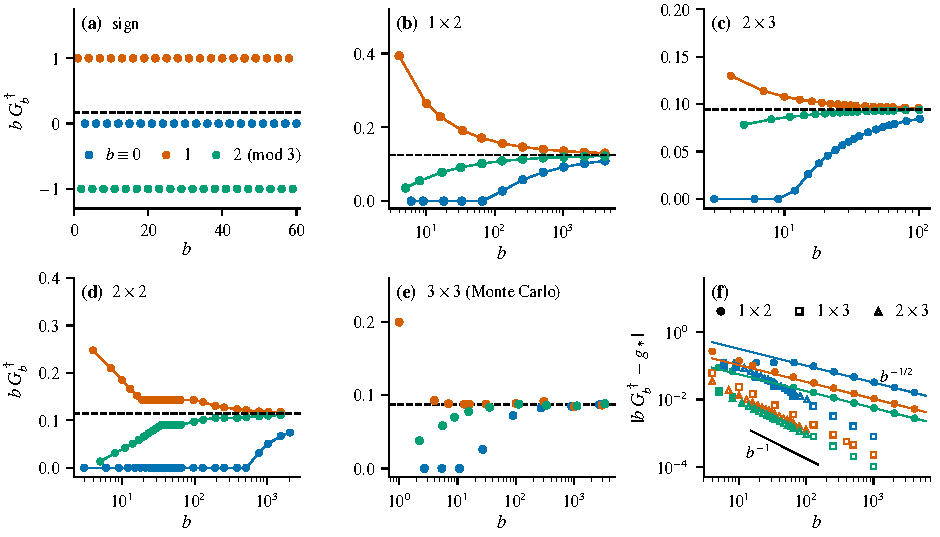
\includegraphics[width=\textwidth]{fig_lattice.pdf}
\caption{The scaled bias $b\,G_b^\st$ (one entry of $\arg\min\psi_{\xi_b}$) for noise with independent entries in
$\{-1,2\}$ of probabilities $\frac23,\frac13$, a lattice law, against the batch size; colours are the residues of $b$
modulo $3$ and the dashed line is the prediction $\gs$. (a) Sign descent: no limit (Theorem~\ref{thm:sign}). (b)--(e)
Euclidean and nuclear geometries: convergence to $\gs$ in every residue class (Theorem~\ref{thm:nuclear}), slowly and
after a transient locking at $0$ for square matrices. (f) Errors for the non-square sizes; lines: the predicted
lattice term $|{\rm coef}|\,b^{-1/2}$ for $1\times2$, and slope $-1$.}
\label{fig:lattice}
\end{figure}

\section{Setting}\label{sec:class}

Throughout, $E$, $\nu$, $o$ are as above, $|\cdot|$ is the Euclidean norm of $E$, and $\Med_\nu(\xi)=-\arg\min\psi_\xi$
is a nonempty convex compact set whenever $\E\nu(\xi)<\infty$. The Gaussian objects \eqref{eq:gstar} are well defined
for every norm: $\Phi_\Sigma$ is smooth and odd, and $J_\Sigma$ is symmetric positive definite (Lemma~\ref{lem:gauss}).

\begin{assumption}[bounded noise]\label{ass:B}\StmtAssB\end{assumption}

For the mean of $b$ samples, $\ew=b^{-1/2}$, $\sqrt{\rho_2}=b^{-1/2}$ and $\rho_3/\rho_2=1/b$. The following class
abstracts what the proofs use.

\begin{definition}[cube expansion]\label{def:class}\StmtClass\end{definition}

\textup{(E2)} is a one-term Edgeworth expansion of the characteristic function on the cube of side $1/\varepsilon$ where
a Taylor expansion is available; \textup{(E1)} is the substitute for Cram\'er's condition. It says nothing about the
size of $\chi_X$ at any given frequency, which may be close to $1$, only that its \emph{mass} in a cube of side
$1/\varepsilon$ is no larger than near the origin.

\begin{proposition}[weighted sums belong to the class]\label{prop:sums-main}
Under Assumption~\ref{ass:B} there is $\varepsilon_0>0$ such that $X_w\in\mathcal X(\ew)$ whenever $\ew\le\varepsilon_0$,
with covariance $\Sigma$, cubic tensor $\cK=\rho_3\rho_2^{-3/2}K_3$ and constants depending only on $N,M,\lambda$.
\end{proposition}

This is Proposition~\ref{prop:sums}. Its key step is the following elementary inequality, in which lattice laws are
the extremal case.

\begin{lemma}[mass of the characteristic function in cubes]\label{lem:cube-main}
Under Assumption~\ref{ass:B} there are $c_1,C_1>0$, depending only on $N,M,\lambda$, such that if $\ew\le\frac12$ then
$\int_{t_0+[-a,a]^N}|\E e^{i\inner t{X_w}}|\,dt\le C_1$ for every $t_0\in E$, with $a=c_1/\ew$.
\end{lemma}

\noindent\emph{Idea of proof.} Split the weights into two halves of comparable energy, so that
$|\chi_{X_w}|\le\frac12(g_A+g_B)$ with $g_A,g_B$ characteristic functions of symmetrized sums, which are
\emph{nonnegative}. For a nonnegative characteristic function $g$ of a vector $Y$ and a tent function $\Delta$ with
nonnegative Fourier transform, $\int g\,\Delta(\cdot-s_0)=\E[e^{i\inner{s_0}Y}\check\Delta(Y)]\le\E\check\Delta(Y)=\int g\,\Delta$:
the translated mass is at most the mass at the origin, which is Gaussian. (Lemma~\ref{lem:cube}.)

\section{The flat case: sign descent fails}\label{sec:sign}

For the $\ell_1$ norm the problem decouples across coordinates, so it suffices to treat $E=\R$.

\begin{theorem}[sign descent with discrete noise]\label{thm:sign}\StmtSign\end{theorem}

The proof (Appendix~\ref{app:sign}) combines Esseen's expansion of the distribution function of a lattice sum, whose
discontinuous term has the same order $b^{-1/2}$ as the skewness term, with the fact that a median is a point where
the distribution function crosses $\frac12$. For entries in $\{-1,2\}$ with probabilities $\frac23,\frac13$ one has
$\gs=\frac16$, $h=3$ and $b\,G_b^\st=0,1,-1$ according to $b\bmod3$: panel (a) of Figure~\ref{fig:lattice}. Part (iii)
is noteworthy: on an integer lattice with moderate skewness, sign descent is \emph{exactly} unbiased for large batches,
whereas the smooth theory predicts a bias $\gs/b$.

\section{Mechanism I: singular sets of codimension at least two}\label{sec:codim}

\begin{assumption}[singular set of codimension $c$]\label{ass:R}\StmtAssR\end{assumption}

The Euclidean norm satisfies it with $V=\{0\}$, $c=N$; a block norm $\sum_g|y_g|$ with $c$ the smallest block size; the
nuclear norm on $\R^{K\times d}$, $K<d$, with $V=\{\rank<K\}$, $\dist(\cdot,V)=\sigma_K$ and $c=d-K+1$
(Lemma~\ref{lem:examples}; the derivative bounds for the polar factor follow from the integral representation
$\polar(M)=\frac2\pi\int_0^\infty(MM^\top+\tau^2I)^{-1}M\,d\tau$).

\begin{theorem}[codimension principle]\label{thm:codim}\StmtCodim\end{theorem}

\noindent\emph{Idea of proof.} For a smooth compactly supported $f$, Fourier inversion, \textup{(E2)} on the central cube
and \textup{(E1)} on its translates give (Lemma~\ref{lem:test})
\begin{equation}\label{eq:test-main}
\Big|\E f(x+X)-\int f(x+y)\psie(y)\,dy\Big|\le C_m\big(\varepsilon^3\|f\|_{L^1}+\varepsilon^m\|D^mf\|_{L^1}\big),\qquad m>N.
\end{equation}
Cut $o$ into a part supported at distance at least $\varepsilon$ from $V$ and a part within $2\varepsilon$ of $V$. For
the first, $\|D^mf\|_{L^1}\lesssim\varepsilon^{c-m}$ by a dyadic decomposition in $\dist(\cdot,V)$, so \eqref{eq:test-main}
gives $\varepsilon^c+\varepsilon^3$. The second is bounded by the probability that $x+X$ is within $2\varepsilon$ of
$V$, which is $O(\varepsilon^c)$ because \textup{(E1)} implies $\Prob(X\in B(y,r))\le C\max(r,\varepsilon)^N$
(Lemma~\ref{lem:ball}): at scale $\varepsilon$ the law of $X$, even on a lattice of mesh $\varepsilon$, is as spread as a
bounded density. Hence $\E\,o(x+X)=\int o(x+y)\psie(y)dy+O(\varepsilon^{\min(c,3)})$, the right-hand side is
$J_\Sigma(x-\hat x)+O(\varepsilon^3)$ near the origin (Lemma~\ref{lem:locate}), and monotonicity of the subdifferential
of a convex function localizes the minimizers. For $c=1$ the bound $\varepsilon^{c}$ is of the order of $\hat x$ itself,
and the argument, correctly, proves nothing. (Appendix~\ref{app:codim}.)

\section{Mechanism II: Fourier decay of the Laplacian of the norm}\label{sec:laplace}

\begin{assumption}[decay]\label{ass:L}\StmtAssL\end{assumption}

Since $\nu$ is convex and homogeneous of degree one, $\Delta\nu$ is a nonnegative measure, homogeneous of degree
$-1$; the cut-off only makes it finite. Assumption~\ref{ass:L} is a quantitative way of saying that the singular set of
$\nu$ is curved in every direction.

\begin{theorem}[curvature and symmetry]\label{thm:laplace}\StmtLaplace\end{theorem}

\noindent\emph{Idea of proof.} Let $h_\delta$ be an even mollifier at scale $\delta=\varepsilon^{q}\ll\varepsilon$. Three
steps. \emph{(1)} For the smoothed, truncated norm $f=(\chi(\cdot/R)\nu)*h_\delta$ we do not use \eqref{eq:test-main} but
the sharper form with $\sum_{j\ne0}\sup_{Q_j}|\widehat f|$ over the cubes $Q_j$ of side $2c_\ast/\varepsilon$: since
$|t|^2\widehat{\chi\nu}(t)=-\widehat{\lambda_\nu}(t)$, Assumption~\ref{ass:L} gives $|\widehat f(t)|\lesssim|t|^{-2-\kappa}$
up to the frequency $1/\delta$, and the sum is of order $\varepsilon^{N}\delta^{-(N-2-\kappa)}=\delta^2$. \emph{(2)} Convexity
removes the mollifier at the level of values, under the true law and without any regularity of it:
\begin{equation}\label{eq:sandwich-main}
2\,\nu*h_\delta-\nu*h_{2\delta}\ \le\ \nu\ \le\ \nu*h_\delta\qquad\text{pointwise},
\end{equation}
while on the comparison side, which is smooth, the mollifier costs $O(\delta^2)$. Thus
$|H-\Psi|\lesssim\delta^2=\varepsilon^{2q}$ (Proposition~\ref{prop:value}). \emph{(3)} If a convex function is within
$\eta$ of a $C^2$ function on a ball, each of its subgradients is within $O(\sqrt\eta)$ of the gradient
(Lemma~\ref{lem:upgrade}); this gives $\varepsilon^{q}$, which is $o(\varepsilon)$ because $q>1$. The exponent
$q=N/(N-\kappa)$ balances the smoothing error $\delta^2$ against the resonances. (Appendix~\ref{app:laplace}.)

\begin{lemma}[symmetry gives decay]\label{lem:sym-main}
\textup{(a)} If $\nu$ is invariant under a compact group $\mathcal G\subset O(E)$ whose orbital integrals satisfy
$\sup_{|e|=|y|=1}|\int_{\mathcal G}e^{iu\inner e{gy}}dg|\le C(1+u)^{-\kappa}$, then $|\widehat{\lambda_\nu}(t)|\le C'(1+|t|)^{-\kappa}$.
\textup{(b)} For $k,l\ge3$ the group $\SO(k)\times\SO(l)$ acting on $\R^{k\times l}$ by $y\mapsto UyV^\top$ satisfies this
with $\kappa=\frac12$; hence every norm invariant under left and right rotations (nuclear, operator, Schatten, Ky Fan
norms) satisfies Assumption~\ref{ass:L} with $\kappa=\frac12$. \textup{(c)} The nuclear norm on $\R^{2\times2}$ satisfies
Assumption~\ref{ass:L} with $\kappa=\frac12$.
\end{lemma}

These are Lemmas~\ref{lem:orbit}, \ref{lem:matrices} and~\ref{lem:twobytwo}. For (b), the phase
$g\mapsto\inner e{gy}$ has, at every point of the group and for all unit $e,y$, a nonvanishing derivative of order one
or two, because products $A_1A_2$ of skew-symmetric matrices of size at least $3$ span all matrices and the mixed
derivatives $AyB$ reach the entries outside the row and column spaces of $y$; van der Corput's lemma then gives the
uniform decay $u^{-1/2}$, which is sharp for $k=l=3$. For size $2$ the orbital bound fails, and (c) is proved by hand:
in the coordinates $y_\pm$ of the conformal and anticonformal parts of a $2\times2$ matrix,
$\nnuc M=\sqrt2\max(|y_+|,|y_-|)$, the measure $\Delta\nu$ is explicit, and its Fourier transform is a superposition of
products of Bessel functions $J_0(|t_+||y_+|)J_0(|t_-||y_-|)$.

\paragraph{Proof of Theorem~\ref{thm:nuclear}.} For $K\ne d$ apply Theorem~\ref{thm:codim} with $c=|K-d|+1$; for
$K=d$ apply Theorem~\ref{thm:laplace} with $N=K^2$, $\kappa=\frac12$, so that $q-1=1/(2K^2-1)$.\hfill$\blacksquare$

\paragraph{Remarks.} (1) Mechanism II covers the operator norm and all Schatten and Ky Fan norms in sizes
$k,l\ge3$, non-square included, though with a worse exponent than mechanism I when the latter applies.
(2) The exponents $\gamma$ for square matrices are what the method gives; we do not claim they are sharp, and
Figure~\ref{fig:lattice}(d),(e) suggests faster convergence after a transient. The transient is real: for small batches
on the residue class where $0$ is a lattice point, the subdifferential of $\psi_{\xi_b}$ at $0$ contains $0$ and the
median is exactly $0$ (for $2\times2$ matrices and the noise of Figure~\ref{fig:lattice}, up to $b=513$).
(3) Theorem~\ref{thm:laplace} controls every subgradient: a rank-deficient argument has positive probability under
discrete noise, and the value of the direction map there is immaterial to first order.

\section{Consequences: momentum, finite sums, sampling without replacement}\label{sec:cons}

\begin{corollary}[batch and momentum together, uniformly in $\beta$]\label{cor:mom}\StmtMomCor\end{corollary}

The exponentially averaged noise is a weighted sum with $\rho_3/\rho_2=1/\beff$ and $\ew^2=\theta$, so this is the
weighted form of the theorems. Note that $\beff$ is not the variance-effective batch size $b(1+\beta)/(1-\beta)$: the
bias is a third-cumulant effect and is averaged differently; the two differ by a factor that tends to $\frac43$ as
$\beta\to1$.

\begin{corollary}[finite sums]\label{cor:fs}\StmtFS\end{corollary}

\begin{theorem}[finite-population bias]\label{thm:wor}\StmtWor\end{theorem}

\noindent\emph{Idea of proof.} A sample without replacement is a vector of independent Bernoulli($p$) inclusion variables
conditioned on their sum. Writing the indicator of the conditioning as a Fourier integral expresses the characteristic
function of $T=b\,\xi_{n,b}/\sqrt v$ as a ratio of integrals of the unconditional characteristic function over one more
frequency variable. The modulus of the latter is bounded by $\exp(-p(1-p)\sum_i(1-\cos s_i))$, the characteristic
function of a symmetrized compound Poisson vector, hence nonnegative definite, and the argument of
Lemma~\ref{lem:cube-main} applies in dimension $N+1$; a Taylor expansion, uniform in $p\in(0,1)$, gives \textup{(E2)}
with $\varepsilon=v^{-1/2}$ and cubic tensor $(1-2p)v^{-1/2}K_{3,n}$. So $T\in\mathcal X(v^{-1/2})$
(Proposition~\ref{prop:worclass}) and Theorems~\ref{thm:codim} and~\ref{thm:laplace} apply verbatim. The factor
$1-2p$ is the skewness of a centred Bernoulli variable; the exact form $(n-2b)/(n-2)$ is the one consistent with the
exact identity $\Med_\nu(\xi_{n,n-b})=-\frac b{n-b}\Med_\nu(\xi_{n,b})$, which holds because the complement of a sample is a
sample. (Appendix~\ref{app:wor}.)

\smallskip
The finite-population correction of the \emph{variance} is $1-p$; the correction of the bias is $1-2p$ to leading
order, and it is negative for $b>n/2$: with large batches drawn without replacement, an orthogonalized step is biased
in the direction \emph{opposite} to the skewness.

\section{Numerical illustrations and sharpness}\label{sec:exp}

The computations are exact evaluations of the convex function $\psi_{\xi_b}$ for lattice noise (the law of the sum is
enumerated; truncated mass below $10^{-8}$), except where Monte Carlo is indicated, in which case standard errors come
from independent batches. Details and scripts are in Appendix~\ref{app:exp} and the supplementary material.

\paragraph{Lattice noise.} Figure~\ref{fig:lattice} and Table~\ref{tab:exact} use independent entries in $\{-1,2\}$ with
probabilities $\frac23,\frac13$. For sign descent the scaled bias is $0,+1,-1$ according to $b\bmod3$ for every $b$
computed, up to $3002$. For the Euclidean and non-square nuclear cases it converges to $\gs$ in all three residue
classes with the exponents of Theorem~\ref{thm:codim}: fitted slopes $-0.51$ ($1\times2$, $c=2$), $-1.00$
($1\times3$, $c=3$) and $-0.98$ to $-1.01$ ($2\times3$, $c=2$, where the rate $b^{-1/2}$ of the theorem is therefore not
attained on this example). For square matrices convergence holds but is slow on the class $b\equiv0$, where $0$ is a
lattice point: for $2\times2$ matrices the minimizer is \emph{exactly} $0$ up to $b=513$, then $0.031$, $0.051$,
$0.067$, $0.074$ at $b=768,1026,1536,2049$, against $\gs=0.1138$; for $3\times3$ matrices the three classes agree
with $\gs$ within Monte-Carlo error at $b\approx3000$. No rate can be read off for the square case; the theorem
guarantees $b^{-1/14}$ and $b^{-1/34}$.

\begin{proposition}[formal; confirmed numerically]\label{prop:lattice2}\StmtLattice\end{proposition}

For the $1\times2$ example the predicted values of $\sqrt b\,(b\,G_b^\st-\gs)$ are $-1.012$, $+0.333$, $-0.178$ for
$b\equiv0,1,2$; the exact values at $b=4098,4096,4097$ are $-1.028$, $+0.337$, $-0.179$. The derivation is in
Appendix~\ref{app:lattice}; we state it as a formal result because we have not controlled the remainder of the lattice
local expansion against the singular kernel.

\begin{table}[t]
\centering\small
\begin{tabular}{@{}lccccc@{}}
\toprule
geometry & $\gs$ & $b\equiv0$ & $b\equiv1$ & $b\equiv2$ & largest $b$\\
\midrule
sign ($1\times1$) & $0.1667$ & $0$ & $+1$ & $-1$ & 3000--3002\\
Euclidean $1\times2$ & $0.1250$ & $0.1089$ & $0.1303$ & $0.1222$ & 4096--4098\\
Euclidean $1\times3$ & $0.1000$ & $0.0992$ & $0.1002$ & $0.0999$ & 1000--1002\\
nuclear $2\times3$ & $0.0947$ & $0.0847$ & $0.0960$ & $0.0937$ & 100--102\\
nuclear $2\times2$ & $0.1138$ & $0.0742$ & $0.1176$ & $0.1111$ & 1537--2049\\
nuclear $3\times3$ & $0.0875$ & $0.0871\pm0.0021$ & $0.0866\pm0.0022$ & $0.0883\pm0.0025$ & 3000--3002\\
\bottomrule
\end{tabular}

\caption{Scaled bias $b\,G_b^\st$ for the lattice noise of Figure~\ref{fig:lattice} at the largest batch sizes computed, by
residue class of $b$ modulo $3$ (exact, except $3\times3$: Monte Carlo with standard errors), and the prediction $\gs$.}
\label{tab:exact}
\end{table}

\begin{figure}[t]
\centering
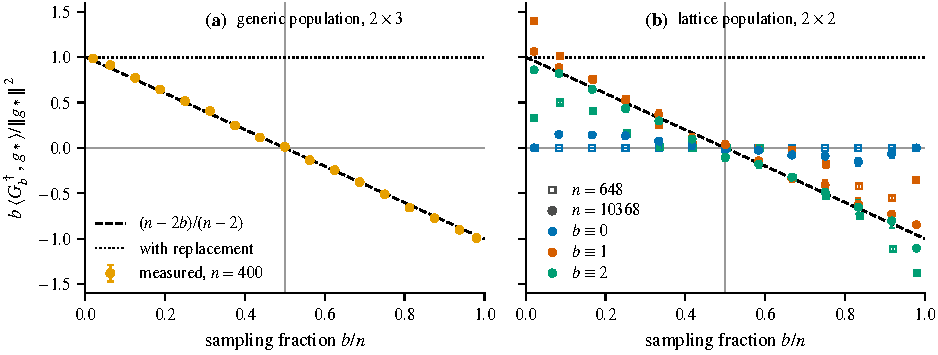
\includegraphics[width=\textwidth]{fig_wor.pdf}
\caption{Sampling without replacement, nuclear norm: the measured coefficient $b\inner{G_b^\st}{\gs}/|\gs|^2$ against the
sampling fraction, with the prediction $(n-2b)/(n-2)$ of Theorem~\ref{thm:wor}. (a) A generic population of $n=400$
matrices of size $2\times3$. (b) Lattice populations of $2\times2$ matrices with entries in $\{-1,2\}$.}
\label{fig:wor}
\end{figure}

\paragraph{Without replacement.} For a generic population (Figure~\ref{fig:wor}a) the coefficient follows
$(n-2b)/(n-2)$ with root-mean-square deviation $0.02$ and changes sign at $b=n/2$. Panel (b) is the hardest case
covered by Theorem~\ref{thm:wor}: a lattice population in the square size $2\times2$, where the guaranteed rate is
$v^{-1/14}$. The sign reversal is visible at both population sizes, and at $n=10368$ the classes $b\equiv1,2$ follow
the line; the class $b\equiv0$ is still mostly locked at $0$, as in Figure~\ref{fig:lattice}(d).

\paragraph{Momentum.} Appendix~\ref{app:exp} (Figure~\ref{fig:mom}) runs the iteration
$M_t=\beta M_{t-1}+(1-\beta)(\nabla F(W_t)+\xi_t)$, $W_{t+1}=W_t-\eta_t\polar(M_t)$ on a quadratic with the same lattice
noise in size $3\times3$. For $\beta\in\{0.5,0.9\}$ and $\beff\ge9$ the limiting gradient multiplied by $\beff$ is within
$5\%$ of $\gs$ (for instance $0.0868\pm0.0013$ at $b=16$, $\beta=0.9$, against $0.0875$), and incompatible with the
variance-effective normalization, which would give $0.066$ to $0.068$. The same experiment with $o=\operatorname{sign}$ shows
that the failure of sign descent is a property of batch means: for $\beta=0$ the limit follows the lattice values of
Theorem~\ref{thm:sign}, but for $\beta\in\{0.5,0.9\}$ it agrees with $\gs/\beff$ ($\beff\times$ limit $=0.168$ to $0.171$
for $b=6,\dots,16$, $\beta=0.5$, against $\frac16$). The exponentially filtered noise is not a lattice law, and
Theorem~\ref{thm:sign}(a) suggests that the law is then restored; we have no proof for filtered noise.

\section{Discussion}\label{sec:disc}

\emph{What decides the validity of the smooth theory is the geometry of the norm, not the arithmetic of the noise.}
For norms whose singular set is flat (the $\ell_1$ norm, and more generally polyhedral norms, whose direction maps
are locally constant) lattice noise is visible at first order. For the nuclear norm it is not, in any size beyond
$1\times1$. Practically, the bias of Muon-type methods on finite data sets is described by the two-moment formula of
\citet{companionI} whatever the arithmetic of the per-sample gradients, with batch size $\beff$ under momentum and with
the factor $(n-2b)/(n-2)$ without replacement.

\emph{Open problems.} (1) The exponents for square matrices: is the remainder $O(b^{-3/2})$, as for $|K-d|=1$? The
decay $\kappa=\frac12$ is sharp for the orbital integrals but the method loses in the passage from values to
subgradients. (2) Sign descent with momentum: the experiment of
Section~\ref{sec:exp} suggests that exponential averaging restores the law for the $\ell_1$ norm; a proof would need a
quantitative non-lattice property of filtered sums. (3) Polyhedral norms other than $\ell_1$, for instance the $\ell_\infty$-operator norms of other steepest
descent methods, should fail as sign descent does; a characterization of the norms for which \eqref{eq:law} holds for
all bounded laws would be interesting, and Assumption~\ref{ass:L} with some $\kappa>0$ is a natural candidate. (4) The
lattice term of Proposition~\ref{prop:lattice2} awaits a proof. (5) Unbounded noise with a few moments, and
parameter-dependent noise, where the companion paper needs a uniform Edgeworth expansion that is so far available
under Cram\'er's condition only.

\bibliography{../../master/shared/refs}

\appendix
\section{The Gaussian side}\label{app:gauss}
% Module: Gaussian side (used by both papers). Labels: lem:gauss
\begin{lemma}[Gaussian side]\label{lem:gauss}
Let $\nu$ be a norm on $E$ with direction map $o$, and $\Sigma\succ0$. Write $\varphi_\Sigma$ for the density of
$Z_\Sigma\sim N(0,\Sigma)$ and $\He^\Sigma_k=(-1)^k\varphi_\Sigma^{-1}D^k\varphi_\Sigma$ for the Hermite tensors.
\begin{enumerate}
\item $\psi_\Sigma$ is $C^\infty$, $\Phi_\Sigma=\nabla\psi_\Sigma$ is odd, and the derivatives of $\Phi_\Sigma$ of every
order are bounded on $E$, uniformly for $\Sigma$ in a compact set of positive definite matrices.
\item For every symmetric $k$-tensor $\cK$ and every $x\in E$,
$\int o(x+y)\inner{\cK}{\He^\Sigma_k(y)}\varphi_\Sigma(y)\,dy=D^k\Phi_\Sigma(x)[\cK]$. In particular
$J_\Sigma=\E[o(Z_\Sigma)\otimes\Sigma^{-1}Z_\Sigma]$ and $T_\Sigma[\cK]=\E[o(Z_\Sigma)\inner{\cK}{\He_3^\Sigma(Z_\Sigma)}]$.
\item The even-order derivatives of $\Phi_\Sigma$ vanish at $0$.
\item $J_\Sigma$ is symmetric positive definite, and $\lambda_{\min}(J_\Sigma)$ is bounded below on compact sets of
positive definite $\Sigma$.
\item $J_{c\Sigma}=c^{-1/2}J_\Sigma$ and $T_{c\Sigma}=c^{-3/2}T_\Sigma$ for $c>0$; hence $\gs(c\Sigma,cK_3)=\gs(\Sigma,K_3)$
and $\gs$ is linear in $K_3$.
\item There is $c_0>0$, uniform on compact sets of $\Sigma$, with $|\Phi_\Sigma(h)|\ge c_0\min(|h|,1)$.
\end{enumerate}
\end{lemma}
\begin{proof}
A norm is Lipschitz, hence differentiable almost everywhere, with gradient $o$ wherever it is differentiable; so
$\nabla\psi_\Sigma(h)=\E\,o(h+Z_\Sigma)=\int o(y)\varphi_\Sigma(y-h)\,dy$ by dominated convergence, and one may
differentiate under the integral any number of times because $o$ is bounded: the $k$-th derivative is bounded by
$\sup|o|\int|D^k\varphi_\Sigma|$. This is (1), and $D_h^k[\varphi_\Sigma(y-h)]=(-1)^kD^k\varphi_\Sigma(y-h)
=\He_k^\Sigma(y-h)\varphi_\Sigma(y-h)$ gives (2) after the change of variable $y\mapsto x+y$. Oddness of $o$ and the
symmetry of $Z_\Sigma$ make $\Phi_\Sigma$ odd, whence (3). (5) follows from $o(tx)=o(x)$:
$\Phi_{c\Sigma}(h)=\Phi_\Sigma(h/\sqrt c)$.

(4) $J_\Sigma=\nabla^2\psi_\Sigma(0)$ is symmetric. Fix $v\ne0$, let
$s=\inner{\Sigma^{-1}v}{Z}/\inner v{\Sigma^{-1}v}$ and $Z'=Z-sv$; these are independent and $s\sim N(0,\tau^2)$ with
$\tau^{-2}=\inner v{\Sigma^{-1}v}$. Then $\psi_\Sigma(tv)+\E\nu(Z)=\E\,\hbar(s+t)$ with $\hbar(\varrho)=\E\nu(Z'+\varrho v)$
convex and $|\varrho|\nu(v)-\E\nu(Z')\le\hbar(\varrho)\le\E\nu(Z')+|\varrho|\nu(v)$. Hence the nondecreasing function
$\hbar'$ goes from $-\nu(v)$ to $\nu(v)$, the measure $d\hbar'$ has total mass $2\nu(v)>0$, and
$\inner{J_\Sigma v}v=\int\varphi_{\tau}\,d\hbar'>0$ because the Gaussian density $\varphi_\tau$ is positive. The lower
bound is uniform by continuity of $\Sigma\mapsto J_\Sigma$ and compactness.

(6) For a unit vector $\hat h$, $t\mapsto\inner{\Phi_\Sigma(t\hat h)}{\hat h}$ is nondecreasing by convexity of
$\psi_\Sigma$, and equals $t\inner{J_\Sigma\hat h}{\hat h}+O(t^3)$ near $0$ by (1) and (3), with uniform constants.
\end{proof}


\section{Fourier comparison in the class $\mathcal X(\varepsilon)$; weighted sums}\label{app:fourier}
% Module: Edgeworth comparison without Cramer's condition.
% Labels: lem:test, lem:ball, lem:cube, lem:near, prop:sums, lem:locate
\begin{lemma}[test functions]\label{lem:test}
Let $X\in\mathcal X(\varepsilon)$ with comparison density $\psie$, and $Q_j=2aj+[-a,a]^N$, $j\in\Z^N$, $a=c_\ast/\varepsilon$.
For every $f\in C_c^\infty(E)$ and every $x\in E$,
\begin{equation}\label{eq:test}
\Big|\E f(x+X)-\int f(x+y)\psie(y)\,dy\Big|\le C\Big(\varepsilon^3\|f\|_{L^1}+\sum_{j\ne0}\sup_{t\in Q_j}|\widehat f(t)|\Big),
\end{equation}
where $\widehat f(t)=\int f(z)e^{-i\inner tz}dz$. Consequently, for every integer $m>N$,
the right-hand side is at most $C_m(\varepsilon^3\|f\|_{L^1}+\varepsilon^m\|D^mf\|_{L^1})$.
\end{lemma}
\begin{proof}
By Fourier inversion, $\E f(x+X)=(2\pi)^{-N}\int\widehat f(t)e^{i\inner tx}\chi_X(t)\,dt$ and likewise for $\psie$ with
$\widehat\psie$ in place of $\chi_X$ ($\widehat f$ is a Schwartz function, $\chi_X$ and $\widehat\psie$ are bounded). On
$Q_0$, $|\widehat f|\le\|f\|_{L^1}$ and \textup{(E2)} bound the difference by $C_\ast\varepsilon^3\|f\|_{L^1}$. Outside
$Q_0$, $|t|\ge c_\ast/\varepsilon$ and $|\widehat\psie(t)|\le C(1+|t|^6)e^{-\lambda|t|^2/2}$, so
$\int_{E\setminus Q_0}|\widehat f||\widehat\psie|\le C\|f\|_{L^1}e^{-c/\varepsilon^2}$; and
$\int_{Q_j}|\widehat f||\chi_X|\le C_\ast\sup_{Q_j}|\widehat f|$ by \textup{(E1)}. For the last claim, $|t|\ge a|j|_\infty$
on $Q_j$ and $|\widehat f(t)|\le N^{m/2}|t|^{-m}\|D^mf\|_{L^1}$ (integrate by parts $m$ times in a coordinate with
$|t_k|\ge|t|/\sqrt N$); $\sum_{j\ne0}|j|_\infty^{-m}<\infty$ for $m>N$.
\end{proof}

\begin{lemma}[small balls and thin neighbourhoods of cones]\label{lem:ball}
Let $X\in\mathcal X(\varepsilon)$. \textup{(i)} $\Prob(X\in B(y,r))\le C\max(r,\varepsilon)^N$ for all $y\in E$, $r>0$.
\textup{(ii)} Let $V\subset E$ be a closed cone with $\vol\{y\in B(0,1):\dist(y,V)\le r\}\le C_Vr^c$ for $r\le1$. Then for
all $x\in E$, $R\ge1$ and $0<r\le R$,
$\Prob\big(|x+X|\le R,\ \dist(x+X,V)\le r\big)\le C\,R^{N-c}\max(r,\varepsilon)^c$.
\end{lemma}
\begin{proof}
(i) Let $k(z)=\prod_{j\le N}(\sin(z_j/2)/(z_j/2))^2$. Then $k\ge(2/\pi)^{2N}$ on $[-\pi,\pi]^N$, and $\widehat k$ is
bounded and supported in $[-1,1]^N$. For $r\ge\varepsilon$,
$\Prob(X\in B(y,r))\le(\pi/2)^{2N}\E\,k((X-y)/r)\le Cr^N\int_{|t|_\infty\le1/r}|\chi_X(t)|\,dt$, and the cube
$[-1/r,1/r]^N$ is covered by at most $(1+\varepsilon/(c_\ast r))^N\le C$ cubes of side $2c_\ast/\varepsilon$; apply
\textup{(E1)}. For $r<\varepsilon$ use monotonicity in $r$.
(ii) Let $\varrho=\max(r,\varepsilon)$ and $\{z_i\}$ a maximal $\varrho$-separated subset of
$A=\{z\in B(0,R):\dist(z,V)\le r\}$. The balls $B(z_i,\varrho/2)$ are disjoint and contained in
$\{z\in B(0,2R):\dist(z,V)\le2\varrho\}$, whose volume is at most $C_V(2R)^{N-c}(2\varrho)^c$ by homogeneity; so there are
at most $CR^{N-c}\varrho^{c-N}$ of them. $A$ is covered by the balls $B(z_i,\varrho)$; apply (i).
\end{proof}

\begin{lemma}[where the comparison field vanishes]\label{lem:locate}
Let $\psie$ be a comparison density as in Definition~\ref{def:class} and
$\Psi(x)=\int(\nu(x+y)-\nu(y))\psie(y)\,dy$. Then $\Psi\in C^\infty$,
$\nabla\Psi(x)=\int o(x+y)\psie(y)\,dy$, the derivatives of $\nabla\Psi$ of every order are bounded on $E$, and
\[
\nabla\Psi(x)=J_\Sigma(x-\hat x)+e(x),\qquad\hat x=-\tfrac16J_\Sigma^{-1}T_\Sigma[\cK],\qquad
|e(x)|\le C_A\varepsilon^3\quad\text{for }|x|\le A\varepsilon,
\]
for every $A\ge1$, with $C_A$ depending only on $A$, $\nu$, $\lambda$, $\Lambda$, $C_\ast$; and $|\hat x|\le C\varepsilon$.
\end{lemma}
\begin{proof}
Write $\widehat r(t)=\sum_\alpha c_\alpha(it)^\alpha$ (even multi-indices, $2\le|\alpha|\le6$, $|c_\alpha|\le C\varepsilon^2$).
Then $\psie=\varphi_\Sigma+\frac16\inner{\cK}{\He^\Sigma_3}\varphi_\Sigma+\sum_\alpha c_\alpha(-\partial)^\alpha\varphi_\Sigma$, and
Lemma~\ref{lem:gauss}(2) gives
$\nabla\Psi=\Phi_\Sigma+\frac16D^3\Phi_\Sigma[\cK]+\sum_\alpha c_\alpha\partial^\alpha\Phi_\Sigma$. By
Lemma~\ref{lem:gauss}(1),(3), for $|x|\le A\varepsilon$: $\Phi_\Sigma(x)=J_\Sigma x+O(|x|^3)$;
$D^3\Phi_\Sigma(x)[\cK]=T_\Sigma[\cK]+O(|\cK||x|^2)$ because $D^4\Phi_\Sigma(0)=0$; and
$\partial^\alpha\Phi_\Sigma(x)=O(|x|)$ for even $\alpha$. With $|\cK|\le C_\ast\varepsilon$ all the remainders are $O(\varepsilon^3)$.
\end{proof}

\paragraph{Weighted sums of bounded vectors.} We now verify that the normalized weighted sums of
Assumption~\ref{ass:B} belong to the class, with no condition on the characteristic function
$\varphi(s)=\E e^{i\inner s\zeta}$.

\begin{lemma}[mass of the characteristic function in cubes]\label{lem:cube}
Under Assumption~\ref{ass:B} there are $c_1,C_1>0$, depending only on $N$, $M$ and $\lambda$, such that if $\ew\le\frac12$,
\[
\int_{t_0+[-a,a]^N}\big|\E e^{i\inner t{X_w}}\big|\,dt\ \le\ C_1\qquad\text{for every }t_0\in E,\qquad a=\frac{c_1}{\ew}.
\]
\end{lemma}
\begin{proof}
With $\zeta'$ an independent copy of $\zeta$,
$|\varphi(u)|^2=\E\cos\inner u{\zeta-\zeta'}\le1-\inner u{\Sigma u}+\frac23M^4|u|^4\le e^{-\lambda|u|^2/2}$ for
$|u|\le u_0:=(3\lambda/4)^{1/2}M^{-2}$ (use $\cos\theta\le1-\theta^2/2+\theta^4/24$ and $|\zeta-\zeta'|\le2M$). Since
$\max_kw_k^2\le\rho_2/4$, the indices can be split into two sets $A,B$ with $\sum_{k\in A}w_k^2\ge\rho_2/4$ and
$\sum_{k\in B}w_k^2\ge\rho_2/4$: fill $A$ until its sum first reaches $\rho_2/4$; it is then at most $\rho_2/2$. With
$s=t/\sqrt{\rho_2}$,
\begin{gather*}
\big|\E e^{i\inner t{X_w}}\big|=\prod_k|\varphi(w_ks)|\le\tfrac12\big(g_A(s)+g_B(s)\big),\\
g_A(s)=\prod_{k\in A}|\varphi(w_ks)|^2=\E e^{i\inner s{Y_A}},\qquad Y_A=\sum_{k\in A}w_k(\zeta_k-\zeta'_k)
\end{gather*}
(the series converges in $L^2$ when there are infinitely many weights). Let $\Delta(s)=\prod_{j\le N}(1-|s_j|/\alpha)_+$
with $\alpha=u_0/(\sqrt N\max_kw_k)$; its Fourier transform
$\check\Delta(y)=\int\Delta(s)e^{i\inner sy}ds=\prod_j\alpha\big(\frac{\sin(\alpha y_j/2)}{\alpha y_j/2}\big)^2$ is
nonnegative. Hence, for every $s_0$, by Fubini,
\begin{align*}
\int g_A(s)\Delta(s-s_0)\,ds&=\E\big[e^{i\inner{s_0}{Y_A}}\check\Delta(Y_A)\big]\le\E\,\check\Delta(Y_A)=\int g_A(s)\Delta(s)\,ds\\
&\le\int e^{-\lambda\rho_2|s|^2/8}ds=\Big(\frac{8\pi}{\lambda\rho_2}\Big)^{N/2},
\end{align*}
because $|w_ks|\le u_0$ on the support of $\Delta$. As $g_A\ge0$ and $\Delta(\cdot-s_0)\ge2^{-N}$ on
$s_0+[-\alpha/2,\alpha/2]^N$, we get $\int_{s_0+[-\alpha/2,\alpha/2]^N}g_A\le2^N(8\pi/\lambda\rho_2)^{N/2}$, and the same for
$g_B$. The change of variables $t=\sqrt{\rho_2}\,s$ gives the claim with $c_1=u_0/(2\sqrt N)$.
\end{proof}

The lemma says that the mass of $|\chi_{X_w}|$ near \emph{any} frequency is at most a constant multiple of its mass near
the origin. The resonances of a lattice law are the worst case, and they are harmless against test functions whose
Fourier transform is summable over a lattice of mesh $1/\ew$.

\begin{lemma}[small frequencies]\label{lem:near}
Under Assumption~\ref{ass:B} let
$\widehat\psie_w(t)=e^{-\inner t{\Sigma t}/2}\big(1+\varepsilon_3p_1(t)+\varepsilon_4p_2(t)+\frac12\varepsilon_3^2p_1(t)^2\big)$ with
$p_1(t)=\frac16K_3[(it)^{\otimes3}]$, $p_2(t)=\frac1{24}K_4[(it)^{\otimes4}]$, $\varepsilon_3=\rho_3\rho_2^{-3/2}$,
$\varepsilon_4=\rho_4\rho_2^{-2}$. There are $c_2\le c_1$ and $C_2$ such that for $|t|_\infty\le c_2/\ew$,
\[
\big|\E e^{i\inner t{X_w}}-\widehat\psie_w(t)\big|\le C_2\,\ew^3\big(|t|^5+|t|^{9}\big)e^{-\lambda|t|^2/4}.
\]
\end{lemma}
\begin{proof}
$|\varphi(u)-1|\le M^2|u|^2/2$, so on $|u|\le1/M$ the function $\log\varphi$ is $C^\infty$ with derivatives bounded in
terms of $M$, and $\log\varphi(u)=-\frac12\inner u{\Sigma u}+\frac16K_3[(iu)^{\otimes3}]+\frac1{24}K_4[(iu)^{\otimes4}]+\varrho(u)$,
$|\varrho(u)|\le C|u|^5$. Summing over $u=w_kt/\sqrt{\rho_2}$ (all of norm at most $\ew|t|$) and using
$\rho_p\rho_2^{-p/2}\le\ew^{p-2}$,
\[
\log\E e^{i\inner t{X_w}}=-\tfrac12\inner t{\Sigma t}+A,\qquad A=\varepsilon_3p_1+\varepsilon_4p_2+R,\qquad
|R|\le C\ew^3|t|^5 .
\]
If $\ew|t|\le\sqrt Nc_2$ with $c_2$ small, then $|A|\le\lambda|t|^2/4$. Now $|e^A-1-A-\frac12A^2|\le\frac16|A|^3e^{|A|}$,
$|A|^3\le C\ew^3|t|^9$, and
$A+\frac12A^2=\varepsilon_3p_1+\varepsilon_4p_2+\frac12\varepsilon_3^2p_1^2+O(\ew^3(|t|^5+|t|^8))$. Multiply by
$e^{-\inner t{\Sigma t}/2}\le e^{-\lambda|t|^2/2}$.
\end{proof}

\begin{proposition}[weighted sums belong to the class]\label{prop:sums}
Under Assumption~\ref{ass:B} there is $\varepsilon_0>0$ such that for every weight sequence with $\ew\le\varepsilon_0$,
$X_w\in\mathcal X(\ew)$ with covariance $\Sigma$, cubic tensor $\cK=\varepsilon_3K_3$, even part
$\widehat r=\varepsilon_4p_2+\frac12\varepsilon_3^2p_1^2$, and constants $C_\ast,c_\ast$ depending only on $N$, $M$,
$\lambda$. Here $\varepsilon_3=\rho_3\rho_2^{-3/2}\le\ew$ and $\varepsilon_4=\rho_4\rho_2^{-2}\le\ew^2$.
\end{proposition}
\begin{proof}
\textup{(E1)} is Lemma~\ref{lem:cube} (cubes of half-side $c_2/\ew\le c_1/\ew$ are contained in cubes of half-side
$c_1/\ew$). \textup{(E2)}: integrate the bound of Lemma~\ref{lem:near} over $|t|_\infty\le c_2/\ew$. \textup{(E3)}:
Hoeffding's inequality for each coordinate of $X_w=\sum_k(w_k/\sqrt{\rho_2})\zeta_k$, since
$\sum_kw_k^2/\rho_2=1$, gives $\Prob(|X_w|>u)\le2Ne^{-u^2/(2NM^2)}$. The bounds on $\cK$ and $\widehat r$ follow from
$|K_3|\le M^3$, $|K_4|\le CM^4$.
\end{proof}


\section{Mechanism I: proofs}\label{app:codim}
% Module: mechanism I, singular sets of codimension >= 2.
% Labels: lem:examples, prop:field, proof of thm:codim
\begin{lemma}[examples]\label{lem:examples}
Assumption~\ref{ass:R} holds for: \textup{(a)} the Euclidean norm on $\R^N$, with $V=\{0\}$, $c=N$; \textup{(b)}
block norms $\nu(y)=\sum_g|y_g|$ over a partition of the coordinates into blocks of sizes $n_g$, with
$V=\bigcup_g\{y_g=0\}$, $c=\min_gn_g$; \textup{(c)} the nuclear norm on $\R^{K\times d}$ with $K<d$ (transpose if $K>d$),
with $o=\polar$, $V=\{\rank<K\}$, $\dist(\cdot,V)=\sigma_K$ and $c=d-K+1$. For the $\ell_1$ norm (sign descent) and for
the nuclear norm on square matrices it holds with $c=1$ only.
\end{lemma}
\begin{proof}
(a), (b): $o(y)=(y_g/|y_g|)_g$ is smooth off $V$ and $0$-homogeneous in each block, so $|D^ko(y)|\le C_k\min_g|y_g|^{-k}$
and $\dist(y,V)=\min_g|y_g|$; the volume bound is elementary. (c) For $MM^\top\succ0$,
\[
\polar(M)=(MM^\top)^{-1/2}M=\frac2\pi\int_0^\infty G_\tau(M)\,d\tau,\qquad G_\tau(M)=A^{-1}M,\quad A=MM^\top+\tau^2I .
\]
With $s=(\sigma_K(M)^2+\tau^2)^{1/2}$ we have $\|A^{-1/2}\|\le1/s$ and $\|A^{-1/2}M\|\le1$ in operator norm. Since
$D(A^{-1})[H]=-A^{-1}(HM^\top+MH^\top)A^{-1}$, the derivative $D^kG_\tau(M)[H,\dots,H]$ is a sum of at most $C_k$ words
$A^{-1}X_1A^{-1}X_2\cdots A^{-1}X_jA^{-1}Y$ with $X_i\in\{HM^\top,MH^\top,HH^\top\}$, $Y\in\{M,H\}$, and $k$ letters $H$
in total. Write each $A^{-1}=A^{-1/2}A^{-1/2}$: there are $2(j+1)$ halves; each letter $M$ or $M^\top$ can be grouped
with an adjacent half of its own into a factor of norm at most $1$, and if $\ell$ is the number of letters $M,M^\top$
then $k+\ell=2j+1$, so exactly $2(j+1)-\ell=k+1$ halves remain, each of norm at most $1/s$. Hence
$\|D^kG_\tau(M)\|\le C_k(\sigma_K^2+\tau^2)^{-(k+1)/2}$ and, integrating in $\tau$ for $k\ge1$,
$\|D^k\polar(M)\|\le C_k'\sigma_K(M)^{-k}$ (the case $k=0$ is trivial). The distance from $M$ to $V$ is $\sigma_K(M)$
(Eckart--Young). Finally, with rows $\varrho_j$ of $M$,
$\sigma_K(M)\ge K^{-1/2}\min_j\dist(\varrho_j,\operatorname{span}\{\varrho_l\}_{l\ne j})$, so $\sigma_K(M)\le r$ forces some
row to lie within $\sqrt Kr$ of the span of the others, a subspace of codimension $d-K+1$ in $\R^d$; given the other
rows this has volume at most $C r^{d-K+1}$ in the unit ball. The last sentence: $o$ jumps across a hypersurface.
\end{proof}

\begin{proposition}[mean field, codimension $\ge2$]\label{prop:field}
Let Assumption~\ref{ass:R} hold with $c\ge2$ and let $X\in\mathcal X(\varepsilon)$, $\varepsilon\le\varepsilon_0$, with
comparison density $\psie$. Then, with $\Le=\log(e/\varepsilon)$,
\[
\sup_{|x|\le1}\Big|\E\,o(x+X)-\int o(x+y)\psie(y)\,dy\Big|\le C\big(\varepsilon^{c}+\varepsilon^3\big)\Le^{N/2}.
\]
\end{proposition}
\begin{proof}
Choose $R=C'\sqrt{\Le}$ with $C'$ so large that $\Prob(|x+X|>R)\le\varepsilon^3$ for $|x|\le1$ (by \textup{(E3)}) and
$\int_{|x+y|>R}|\psie(y)|dy\le\varepsilon^3$. Let $\chi_R=\chi(\cdot/R)$ with $\chi\in C_c^\infty(B(0,2))$, $\chi=1$ on
$B(0,1)$, and let $\Theta\in C^\infty(E)$, $0\le\Theta\le1$, with $\Theta=1$ on $\{\dist(\cdot,V)\le\varepsilon\}$,
$\Theta=0$ on $\{\dist(\cdot,V)\ge2\varepsilon\}$, $|D^k\Theta|\le C_k\varepsilon^{-k}$ (mollify the indicator of
$\{\dist\le\frac32\varepsilon\}$ at scale $\varepsilon/4$). Write $o=F_1+F_2+F_3$ with $F_1=o(1-\Theta)\chi_R$,
$F_2=o\,\Theta\chi_R$, $F_3=o(1-\chi_R)$.

$F_3$: both $\E|F_3(x+X)|$ and $\int|F_3(x+y)||\psie(y)|dy$ are at most $C\varepsilon^3$.

$F_2$: $\E|F_2(x+X)|\le\sup|o|\,\Prob(|x+X|\le2R,\ \dist(x+X,V)\le2\varepsilon)\le CR^{N-c}\varepsilon^c$ by
Lemma~\ref{lem:ball}(ii), and $\int|F_2(x+y)||\psie(y)|dy\le C\vol\{z\in B(0,2R):\dist(z,V)\le2\varepsilon\}\le CR^{N-c}\varepsilon^c$.

$F_1\in C_c^\infty(E)$: on its support $\dist(z,V)\ge\varepsilon$, and by Leibniz' rule and Assumption~\ref{ass:R},
$|D^mF_1(z)|\le C_m(\dist(z,V)^{-m}+1)$. Summing over the layers $\{2^i\varepsilon\le\dist(\cdot,V)<2^{i+1}\varepsilon\}$,
$i\ge0$, inside $B(0,2R)$,
\[
\|D^mF_1\|_{L^1}\le C\sum_{i\ge0}(2^i\varepsilon)^{-m}R^{N-c}(2^{i+1}\varepsilon)^c+CR^N\le C\big(R^{N-c}\varepsilon^{c-m}+R^N\big)
\]
for $m=N+1>c$.
Lemma~\ref{lem:test} then gives an error $C(\varepsilon^3R^N+\varepsilon^cR^{N-c}+\varepsilon^mR^N)$ for $F_1$ (apply it to
each coordinate). Summing the three contributions proves the claim.
\end{proof}

\begin{proof}[Proof of Theorem~\ref{thm:codim}]
Let $H(x)=\E[\nu(x+X)-\nu(X)]$, a convex function with $\E\,o(x+X)\in\partial H(x)$. By Proposition~\ref{prop:field}
and Lemma~\ref{lem:locate}, uniformly for $|x|\le A\varepsilon$,
\[
\E\,o(x+X)=J_\Sigma(x-\hat x)+e_1(x),\qquad|e_1(x)|\le C_1\varepsilon^{\min(c,3)}\Le^{N/2}.
\]
Let $\varrho=2C_1\varepsilon^{\min(c,3)}\Le^{N/2}/\lambda_{\min}(J_\Sigma)$, which is at most $\varepsilon$ for
$\varepsilon$ small, and take $A$ with $|\hat x|+\varepsilon\le A\varepsilon$. For $|u|=1$,
$\inner{\E\,o(\hat x+\varrho u+X)}{u}\ge\lambda_{\min}(J_\Sigma)\varrho-C_1\varepsilon^{\min(c,3)}\Le^{N/2}>0$. If a minimizer
$x'$ of $H$ had $|x'-\hat x|>\varrho$, put $u=(x'-\hat x)/|x'-\hat x|$ and $y=\hat x+\varrho u$: the subgradient
inequality gives $H(x')\ge H(y)+(|x'-\hat x|-\varrho)\inner{\E\,o(y+X)}u>H(y)$, a contradiction. Hence
$\arg\min H\subset B(\hat x,\varrho)$, which is the first claim. For weighted sums, Proposition~\ref{prop:sums} gives
$X_w\in\mathcal X(\ew)$ with $\cK=\varepsilon_3K_3$, so $\hat x=\varepsilon_3\gs$; and
$\psi_{\xi_w}(G)=\sqrt{\rho_2}\,H(G/\sqrt{\rho_2})$ with $\sqrt{\rho_2}\,\varepsilon_3=\rho_3/\rho_2$.
\end{proof}


\section{Mechanism II: proofs}\label{app:laplace}
% Module: mechanism II, Fourier decay of the Laplacian of the norm.
% Labels: prop:value, lem:upgrade, proof of thm:laplace, lem:orbit, lem:matrices, lem:twobytwo
Throughout this part $\chi\in C_c^\infty(B(0,2))$ is a fixed radial function with $0\le\chi\le1$ and $\chi=1$ on $B(0,1)$,
$\mu=\Delta\nu$ and $\lambda_\nu=\Delta(\chi\nu)$ in the sense of distributions.

\begin{lemma}[the Laplacian of a norm]\label{lem:lapmeasure}
$\mu$ is a nonnegative Radon measure with $\mu(B(0,s))=s^{N-1}\mu(B(0,1))$, and
$\lambda_\nu=\chi\mu+(2\inner{\nabla\chi}{\nabla\nu}+\nu\Delta\chi)\,dz$ is a finite signed measure supported in
$\overline{B(0,2)}$ with $|\lambda_\nu|(B(0,s))\le Cs^{N-1}$ for $s>0$. With $F_R(z)=\chi(z/R)\nu(z)$, $R\ge1$,
\[
\widehat{F_R}(t)=R^{N+1}\widehat{F_1}(Rt),\qquad|t|^2\widehat{F_1}(t)=-\widehat{\lambda_\nu}(t),\qquad
\|F_R\|_{L^1}\le CR^{N+1}.
\]
Consequently, under Assumption~\ref{ass:L}, $|\widehat{F_R}(t)|\le CR^{N+1}(1+R|t|)^{-2-\kappa}$.
\end{lemma}
\begin{proof}
A convex function has a distributional Hessian which is a nonnegative matrix-valued measure (mollify: the Hessians of
$\nu*h_s$ are nonnegative and converge weakly); its trace is $\mu$. Since $\nu(sz)=s\nu(z)$, the distribution $\mu$ is
homogeneous of degree $-1$, which gives the scaling. The product rule gives the formula for $\lambda_\nu$; the two
last terms are bounded and supported in $\{1\le|z|\le2\}$. The identities for $F_R$ are the dilation rule
$F_R(z)=RF_1(z/R)$ and $\widehat{\Delta f}=-|t|^2\widehat f$. Finally $|\widehat{F_1}(t)|\le\|F_1\|_{L^1}$ for $|t|\le1$
and $|\widehat{F_1}(t)|=|t|^{-2}|\widehat{\lambda_\nu}(t)|$ for $|t|\ge1$.
\end{proof}

\begin{proposition}[comparison of potentials]\label{prop:value}
Let Assumption~\ref{ass:L} hold and $X\in\mathcal X(\varepsilon)$, $\varepsilon\le\varepsilon_0$, with comparison density
$\psie$. Let $H(x)=\E[\nu(x+X)-\nu(X)]$ and $\Psi(x)=\int(\nu(x+y)-\nu(y))\psie(y)\,dy$. Then, with
$q=N/(N-\kappa)$ and $\Le=\log(e/\varepsilon)$,
\[
\sup_{|x|\le2}|H(x)-\Psi(x)|\le C\,\varepsilon^{2q}\,\Le^{(N+1)/2}.
\]
\end{proposition}
\begin{proof}
Let $h\in C_c^\infty(B(0,1))$ be even, nonnegative, of integral one, $h_s=s^{-N}h(\cdot/s)$, $\delta=\varepsilon^q$
(so $\varepsilon\ge\delta$) and $R=C'\sqrt{\Le}$.

\emph{Step 1: smoothed, truncated norm.} Let $f=F_R*h_s$ with $s\in\{\delta,2\delta\}$. Then $f\in C_c^\infty$,
$\|f\|_{L^1}\le CR^{N+1}$ and $|\widehat f(t)|=|\widehat{F_R}(t)||\widehat h(st)|\le C_DR^{N+1}(1+R|t|)^{-2-\kappa}(1+s|t|)^{-D}$
for any $D$, by Lemma~\ref{lem:lapmeasure}. On $Q_j$, $j\ne0$, we have $|t|\ge c_\ast|j|_\infty/\varepsilon$, so by
Lemma~\ref{lem:test}
\[
\Big|\E f(x+X)-\!\int\! f(x+y)\psie(y)dy\Big|\le C\varepsilon^3R^{N+1}+CR^{N-1-\kappa}\varepsilon^{2+\kappa}\sum_{j\ne0}\frac{(1+s|j|/\varepsilon)^{-D}}{|j|^{2+\kappa}}.
\]
Since $2+\kappa<N$, the sum over $|j|\le\varepsilon/s$ is at most $C(\varepsilon/s)^{N-2-\kappa}$, and so is the sum over
$|j|>\varepsilon/s$ when $D>N$. The second term is therefore at most
$CR^{N-1-\kappa}\varepsilon^{N}s^{-(N-2-\kappa)}\le CR^{N-1-\kappa}\delta^{N-\kappa}\delta^{-(N-2-\kappa)}=CR^{N-1-\kappa}\delta^2$,
because $\varepsilon^N=\delta^{N-\kappa}$. Also $\varepsilon^3\le\delta^2$, since $2q\le3$ is equivalent to $N\ge3\kappa$.

\emph{Step 2: removing the truncation.} For $|x|\le2$,
$|(\nu*h_s-F_R*h_s)(z)|\le C(1+|z|)\mathbf 1\{|z|\ge R-1\}$; by \textup{(E3)} and the Gaussian tails of $\psie$, both
$\E$ and $\int\cdot\,|\psie|$ of this function at $x+\cdot$ are at most $\varepsilon^3$ if $C'$ is large. Hence
\begin{align*}
\E(\nu*h_s)(x+X)&=\int(\nu*h_s)(x+y)\psie(y)\,dy+O(R^{N+1}\delta^2)\\&=(\Pi*h_s)(x)+O(R^{N+1}\delta^2),
\end{align*}
where $\Pi(x)=\int\nu(x+y)\psie(y)dy$. $\Pi$ is smooth with bounded second derivatives (Lemma~\ref{lem:locate}) and
$h_s$ is even, so $(\Pi*h_s)(x)=\Pi(x)+O(s^2)$.

\emph{Step 3: convexity removes the smoothing.} For every $z\in E$,
\begin{equation}\label{eq:sandwich}
2(\nu*h_\delta)(z)-(\nu*h_{2\delta})(z)\ \le\ \nu(z)\ \le\ (\nu*h_\delta)(z).
\end{equation}
The right inequality is Jensen's ($h_\delta$ is even with integral one). The left one: $2\nu(z-u)\le\nu(z)+\nu(z-2u)$
by convexity; integrate against $h_\delta(u)\,du$ and note $\int\nu(z-2u)h_\delta(u)du=(\nu*h_{2\delta})(z)$. Taking the
expectation of \eqref{eq:sandwich} at $z=x+X$ under the \emph{true} law of $X$, and using Step 2 for both
$s=\delta$ and $s=2\delta$,
$\E\nu(x+X)=\Pi(x)+O(R^{N+1}\delta^2)$ for $|x|\le2$. Subtract the same identity at $x=0$.
\end{proof}

Step 3 is the point where atoms cease to matter: no smoothness of the law of $X$ and no positivity of the signed
density $\psie$ are used, only the convexity of $\nu$.

\begin{lemma}[from values to subgradients]\label{lem:upgrade}
Let $H$ be convex on $B(0,2)\subset E$, $\Psi\in C^2$ with $\|D^2\Psi\|\le C_2$ there, and
$\sup_{B(0,2)}|H-\Psi|\le\eta\le1$. Then for every $|x|\le1$ and every $v\in\partial H(x)$,
$|v-\nabla\Psi(x)|\le(2+C_2/2)\sqrt\eta$.
\end{lemma}
\begin{proof}
For $|u|=1$ and $d=\sqrt\eta$: $\inner vu\le(H(x+du)-H(x))/d\le(\Psi(x+du)-\Psi(x))/d+2\eta/d\le
\inner{\nabla\Psi(x)}u+C_2d/2+2\eta/d$. Apply this to $u$ and $-u$.
\end{proof}

\begin{proof}[Proof of Theorem~\ref{thm:laplace}]
By Proposition~\ref{prop:value} and Lemma~\ref{lem:upgrade}, with $d_\varepsilon=\varepsilon^q\Le^{(N+1)/4}$,
\begin{equation}\label{eq:allsub}
\sup_{|x|\le1}\ \sup_{v\in\partial H(x)}|v-\nabla\Psi(x)|\le C_1d_\varepsilon .
\end{equation}
By Lemma~\ref{lem:locate}, $\nabla\Psi(x)=J_\Sigma(x-\hat x)+O(\varepsilon^3)$ for $|x|\le A\varepsilon$, and
$\varepsilon^3\le d_\varepsilon\le\varepsilon$ for $\varepsilon$ small because $1<q\le\frac32$. Let
$\varrho=3C_1d_\varepsilon/\lambda_{\min}(J_\Sigma)$. For $|u|=1$, every $v\in\partial H(\hat x+\varrho u)$ has
$\inner vu\ge\lambda_{\min}(J_\Sigma)\varrho-2C_1d_\varepsilon>0$. A minimizer $x'$ of $H$ with $|x'-\hat x|>\varrho$ would
contradict the subgradient inequality at $y=\hat x+\varrho u$, $u=(x'-\hat x)/|x'-\hat x|$:
$H(x')\ge H(y)+(|x'-\hat x|-\varrho)\inner vu>H(y)$. Minimizers exist since $H(x)\ge\nu(x)-2\E\nu(X)$. The statement for
weighted sums follows from Proposition~\ref{prop:sums} as in the proof of Theorem~\ref{thm:codim}.
\end{proof}

\begin{lemma}[symmetry gives decay]\label{lem:orbit}
Let $N\ge2$ and let $\mathcal G\subset O(E)$ be a compact group, with normalized Haar measure $dg$, such that $\nu\circ g=\nu$
for $g\in\mathcal G$ and, for some $0<\kappa\le1$,
\begin{equation}\label{eq:orbital}
\sup_{|e|=|y|=1}\Big|\int_{\mathcal G}e^{iu\inner e{gy}}dg\Big|\le C(1+u)^{-\kappa}\qquad(u\ge0).
\end{equation}
Then $|\widehat{\lambda_\nu}(t)|\le C'(1+|t|)^{-\kappa}$.
\end{lemma}
\begin{proof}
$\nu$, $\chi$ and the Laplacian are $\mathcal G$-invariant, hence so is $\lambda_\nu$, and
$\widehat{\lambda_\nu}(t)=\int\!\int_{\mathcal G}e^{-i\inner t{gz}}dg\,d\lambda_\nu(z)$. By \eqref{eq:orbital} and
Lemma~\ref{lem:lapmeasure},
\[
|\widehat{\lambda_\nu}(t)|\le C\int(1+|t||z|)^{-\kappa}d|\lambda_\nu|(z)\le C\sum_{i\ge-1}(1+|t|2^{-i-1})^{-\kappa}2^{-i(N-1)}
\le C'(1+|t|)^{-\kappa},
\]
summing over the annuli $\{2^{-i-1}<|z|\le2^{-i}\}$ and using $N-1\ge\kappa$.
\end{proof}

\begin{lemma}[left and right rotations]\label{lem:matrices}
Let $k,l\ge3$. The group $\mathcal G=\SO(k)\times\SO(l)$ acting on $\R^{k\times l}$ by $y\mapsto Uy V^\top$ satisfies
\eqref{eq:orbital} with $\kappa=\frac12$. Consequently every norm on $\R^{k\times l}$ that is invariant under left and
right rotations (the nuclear norm, the operator norm, all Schatten and Ky Fan norms) satisfies
Assumption~\ref{ass:L} with $\kappa=\frac12$.
\end{lemma}
\begin{proof}
Fix unit $e,y$ and a point $g_0=(U_0,V_0)$, and consider the phase $\phi(g)=\inner e{gy}$ in the chart
$(A,B)\mapsto(U_0e^{A},V_0e^{B})$, $A\in\mathfrak{so}(k)$, $B\in\mathfrak{so}(l)$. Replacing $e$ by $U_0^\top eV_0$ we may
take $g_0$ to be the identity. The first and second derivatives of $\phi$ at the origin of the chart are the numbers
$\inner e{\mathcal Dy}$, where $\mathcal D$ ranges over the linear span $\mathfrak D$ of the maps
\[
y\mapsto Ay,\quad y\mapsto yB,\quad y\mapsto A_1A_2y,\quad y\mapsto yB_1B_2,\quad y\mapsto AyB,
\]
with $A,A_i\in\mathfrak{so}(k)$ and $B,B_i\in\mathfrak{so}(l)$.
We claim that $\{\mathcal Dy:\mathcal D\in\mathfrak D\}=\R^{k\times l}$ for every $y\ne0$. With the matrix units
$E_{ij}$ and $A_{ij}=E_{ij}-E_{ji}$, one has $A_{ih}A_{hj}=-E_{ij}$ for distinct $i,h,j$ and
$A_{ij}^2=-(E_{ii}+E_{jj})$; as the size is at least $3$, products of two skew matrices span all square matrices. So the
span contains $Cy$ and $yD$ for all $C\in\R^{k\times k}$, $D\in\R^{l\times l}$. Choose orthonormal bases in which
$y=\sum_{i\le r}s_iE_{ii}$, $s_i>0$ (conjugation preserves the skew matrices). Then $Cy$ and $yD$ give every $E_{pq}$
with $q\le r$ or $p\le r$; and for $p,q>r$ and any $i\le r$, $A_{pi}\,y\,A_{iq}=s_iE_{pi}A_{iq}=s_iE_{pq}$. This proves the
claim, so for every unit $e$ some derivative of $\phi$ of order one or two at $g_0$ is nonzero. By continuity and
compactness of $\{|e|=1\}\times\{|y|=1\}\times\mathcal G$ there are $\eta>0$ and a finite atlas such that at every point
some coordinate derivative of order one or two has modulus at least $\eta$ on a coordinate ball of fixed radius, while
the $C^3$ norms of $\phi$ in the charts are bounded uniformly in $(e,y)$. With a partition of unity subordinate to the
atlas, the van der Corput estimate in several variables \citep[Ch.~VIII, \S2.2, Prop.~5]{stein}, whose constant depends
only on the lower bound $\eta$, the order of the derivative and the $C^{3}$ norm of the phase, gives
$|\int_{\mathcal G}e^{iu\phi}dg|\le Cu^{-1/2}$ uniformly. The consequence is Lemma~\ref{lem:orbit}.
\end{proof}

The exponent $\frac12$ of Lemma~\ref{lem:matrices} cannot be improved in general: for $k=l=3$ and $e=y=I/\sqrt3$ the
orbital integral is $\E e^{iu\tr(U)/3}$ for a Haar rotation $U$, and $\tr U=1+2\cos\theta$ has a density with a
non-degenerate critical value, so the integral is of exact order $u^{-1/2}$. For size $2$ the lemma fails
($\SO(2)\times\SO(2)$ fixes the two planes of $2\times2$ matrices described next, and for $e$ in one and $y$ in the other the
orbital integral is identically $1$), but Assumption~\ref{ass:L} still holds:

\begin{lemma}[$2\times2$ matrices]\label{lem:twobytwo}
For $M=\begin{psmallmatrix}p&q\\r&s\end{psmallmatrix}$ let $y_+=\frac1{\sqrt2}(p+s,\,q-r)$ and
$y_-=\frac1{\sqrt2}(p-s,\,q+r)$. Then $M\mapsto(y_+,y_-)$ is an isometry of $(\R^{2\times2},\nF\cdot)$ onto
$\R^2\times\R^2$, $\det M=\frac12(|y_+|^2-|y_-|^2)$,
\[
\nnuc M=\sqrt2\max(|y_+|,|y_-|),\qquad
\polar(M)=\begin{cases}\sqrt2\,\big(y_+/|y_+|,\,0\big)&\text{if }|y_+|>|y_-|,\\[2pt]
\sqrt2\,\big(0,\,y_-/|y_-|\big)&\text{if }|y_-|>|y_+|,\end{cases}
\]
and the nuclear norm on $\R^{2\times2}$ satisfies Assumption~\ref{ass:L} with $N=4$, $\kappa=\frac12$.
\end{lemma}
\begin{proof}
The first three assertions are direct computations: $|y_+|^2+|y_-|^2=p^2+q^2+r^2+s^2$,
$|y_+|^2-|y_-|^2=2(ps-qr)$, and $\nnuc M^2=\nF M^2+2|\det M|=2\max(|y_+|^2,|y_-|^2)$; the formula for the polar factor
is the gradient of $\nnuc\cdot$ on the open sets $\Omega_\pm=\{\pm\det>0\}$. Let $V=\{|y_+|=|y_-|\}$; $V\setminus\{0\}$ is a
smooth hypersurface with unit normal $n=(y_+,-y_-)/|y|$ pointing into $\Omega_+$. On $\Omega_\pm$,
$\nu=\sqrt2|y_\pm|$ is smooth with $\Delta\nu=\sqrt2/|y_\pm|\le2/|y|$, and across $V$ the gradient jumps by
$\sqrt2(\hat y_+,-\hat y_-)$, so that (Green's formula on $E\setminus B(0,\varrho)$, $\varrho\to0$)
\[
\mu=\Delta\nu=\sqrt2\Big(\frac{\mathbf 1_{\Omega_+}}{|y_+|}+\frac{\mathbf 1_{\Omega_-}}{|y_-|}\Big)dy+2\,dS_V .
\]
The rotations of $y_+$ alone and of $y_-$ alone are isometries of $E$ preserving $\nu$, $\chi$, $V$ and $dS_V$, hence
$\lambda_\nu$. Averaging over both,
$\widehat{\lambda_\nu}(t)=\int J_0(|t_+||y_+|)\,J_0(|t_-||y_-|)\,d\lambda_\nu(y)$ with $J_0$ the Bessel function,
$|J_0(u)|\le C(1+u)^{-1/2}$. Choose $\varsigma\in\{+,-\}$ with $|t_\varsigma|\ge|t|/\sqrt2$ and let $\varsigma'$ be the other
sign; then $|\widehat{\lambda_\nu}(t)|\le C\int(1+|t||y_\varsigma|)^{-1/2}d|\lambda_\nu|(y)$, where
$|\lambda_\nu|\le C\mathbf 1_{\{|y|\le2\}}\big[(1+|y_+|^{-1}+|y_-|^{-1})dy+dS_V\big]$. The four contributions are at most
$C|t|^{-1/2}$: the bounded density and the term $|y_{\varsigma'}|^{-1}$ because
$\int_{|y_\varsigma|\le2}(|t||y_\varsigma|)^{-1/2}d^2y_\varsigma\le C|t|^{-1/2}$ and
$\int_{|y_{\varsigma'}|\le2}(1+|y_{\varsigma'}|^{-1})d^2y_{\varsigma'}<\infty$; the term $|y_\varsigma|^{-1}$ because
$\int_{|y_\varsigma|\le2}|y_\varsigma|^{-1}(|t||y_\varsigma|)^{-1/2}d^2y_\varsigma\le C|t|^{-1/2}$; and the surface term because
$|y_\varsigma|=|y|/\sqrt2$ on $V$ and $dS_V=c\,\varrho^2d\varrho\,d\theta_+d\theta_-$ in the coordinates
$y_\pm=\frac{\varrho}{\sqrt2}(\cos\theta_\pm,\sin\theta_\pm)$. Since also $|\widehat{\lambda_\nu}|\le|\lambda_\nu|(E)<\infty$,
$|\widehat{\lambda_\nu}(t)|\le C(1+|t|)^{-1/2}$, and $2+\frac12<4$.
\end{proof}

So a Muon-type step on a $2\times2$ matrix normalizes the larger of the conformal and anticonformal parts of its
argument, and the singular set $\{\det=0\}$ is the cone over a Clifford torus.

% Module: proofs of thm:nuclear, cor:mom (uniform in beta), cor:fs
\begin{proof}[Proof of Theorem~\ref{thm:nuclear}]
If $K\ne d$, Lemma~\ref{lem:examples}(c) gives Assumption~\ref{ass:R} with $c=|K-d|+1\ge2$ (for $K=1$ or $d=1$ the nuclear
norm is the Euclidean norm of $\R^N$, $N\ge2$, and $c=N=|K-d|+1$), and Theorem~\ref{thm:codim} applies:
$\min(c,3)-1=2\gamma$. If $K=d=2$, Lemma~\ref{lem:twobytwo} gives Assumption~\ref{ass:L} with $N=4$, $\kappa=\frac12$; if
$K=d\ge3$, Lemma~\ref{lem:matrices} gives it with $N=K^2$, $\kappa=\frac12$; in both cases Theorem~\ref{thm:laplace}
applies and $q-1=\frac{\kappa}{N-\kappa}=2\gamma$. Finally $\sqrt{\rho_2}\,\ew=\max_kw_k$, which is $1/b$ for a batch mean.
\end{proof}

\begin{proof}[Proof of Corollary~\ref{cor:mom}]
$N_\beta=\xi_w$ for the weights $(1-\beta)\beta^k/b$, each repeated $b$ times: $\rho_p=(1-\beta)^pb^{1-p}/(1-\beta^p)$,
so $\rho_3/\rho_2=1/\beff$, $\ew^2=(1-\beta^2)/b=\theta$ and $\max_kw_k=(1-\beta)/b\le3/\beff$. Apply
\eqref{eq:codimw} or \eqref{eq:laplacew}.
\end{proof}

\begin{proof}[Proof of Corollary~\ref{cor:fs}]
Theorem~\ref{thm:nuclear} applied to $\zeta=\nabla f_I(W)-\nabla F(W)$, which is bounded, centred, with covariance
positive definite exactly when the $n$ gradients affinely span $E$. If $n=N+1$, the differences
$\nabla f_i(W)-\nabla f_1(W)$, $i\ge2$, form a basis of $E$ and generate a lattice that contains the support of
$\zeta-\zeta'$: the law of $\zeta$ is a lattice law.
\end{proof}


\section{Sign descent: proof of Theorem~\ref{thm:sign}}\label{app:sign}
% Module: the flat case (sign descent). Label: proof of thm:sign
\begin{proof}[Proof of Theorem~\ref{thm:sign}]
$b\,G^\st_b=-\{\text{medians of }S_b\}$. \textup{(a)} Esseen's theorem for non-lattice laws with three moments
\citep{esseen,gk}: uniformly in $x$,
$\Prob(S_b\le x\sigma\sqrt b)=\Phi(x)+\frac{\kappa_3}{6\sigma^3\sqrt b}(1-x^2)\varphi(x)+o(b^{-1/2})$, with $\Phi,\varphi$
the standard normal distribution function and density. At $x=m/(\sigma\sqrt b)$ with $m$ bounded this reads
$\frac12+\frac{\varphi(0)}{\sigma\sqrt b}(m+\gs)+o(b^{-1/2})$, and the same holds for $\Prob(S_b<m)$; so every
median $m_b$ of $S_b$ satisfies $m_b+\gs\to0$ (medians are bounded, by the same expansion at $|m|$ large).

\textup{(b)} Esseen's expansion for lattice laws \citep[\S43]{gk} reads, uniformly in $x$,
\[
\Prob(S_b\le x\sigma\sqrt b)=\Phi(x)+\frac{\kappa_3(1-x^2)}{6\sigma^3\sqrt b}\varphi(x)+\frac h{\sigma\sqrt b}\,
S_1\Big(\frac{x\sigma\sqrt b-ba}{h}\Big)\varphi(x)+o(b^{-1/2}),
\]
where $S_1(y)=\lfloor y\rfloor-y+\tfrac12$.
At a point $m\in ba+h\Z$ of the lattice carrying $S_b$, $S_1=\frac12$, and immediately to the left of the next lattice
point $S_1\to-\frac12$. Hence, for bounded $m\in ba+h\Z$,
\begin{align*}
\Prob(S_b\le m)&=\tfrac12+\tfrac{\varphi(0)}{\sigma\sqrt b}\big(m+\gs+\tfrac h2\big)+o(b^{-1/2}),\\
\Prob(S_b<m)=\Prob(S_b\le m-h)&=\tfrac12+\tfrac{\varphi(0)}{\sigma\sqrt b}\big(m+\gs-\tfrac h2\big)+o(b^{-1/2}).
\end{align*}
A lattice point $m$ is a median if and only if $\Prob(S_b<m)\le\frac12\le\Prob(S_b\le m)$, and a point off the lattice
is a median only if it lies between two consecutive lattice medians. So for $b$ large every median lies in
$[-\gs-\frac h2-\delta,-\gs+\frac h2+\delta]$, and a lattice point with $|m+\gs|\le\frac h2-\delta$ has
$\Prob(S_b<m)<\frac12<\Prob(S_b\le m)$, hence is the unique median. \textup{(i)} follows from Weyl's
equidistribution of $ba/h$ modulo $1$. \textup{(ii)}: $\Lambda_b$ depends on $b$ modulo $q$ only; if $q\ge2$ the cosets
are distinct, at most one of them has $\gs$ at the midpoint between two of its points, and the nearest points of two
different cosets differ, so there is no limit; if $q=1$, $\Lambda_b=h\Z$. \textup{(iii)}: $a=0$ and $|\gs|<h/2$.
\end{proof}


\section{Sampling without replacement: proofs}\label{app:wor}
% Module: sampling without replacement. Labels: prop:worclass, proof of thm:wor
\begin{proposition}[the conditional law belongs to the class]\label{prop:worclass}
In the setting of Theorem~\ref{thm:wor} let $h=\sqrt v$ and $T=b\,\xi_{n,b}/h$. There is $v_0$ such that for $v\ge v_0$,
$T\in\mathcal X(1/h)$ with covariance $\Sigma_n$, cubic tensor $\cK=\frac{1-2p}{h}K_{3,n}$, and constants
$\lambda,\Lambda=M^2,C_\ast,c_\ast$ depending only on $N,M,\lambda$.
\end{proposition}
\begin{proof}
Let $I_1,\dots,I_n$ be independent Bernoulli variables of parameter $p=b/n$, $r=p(1-p)$, so $h^2=nr$, and
\[
T'=\frac1h\sum_i(I_i-p)z_i,\qquad C'=\sum_i(I_i-p)=\sum_iI_i-b\ \in\Z .
\]
Conditionally on $C'=0$ the set $\{i:I_i=1\}$ is uniform among subsets of size $b$, and since $\sum_iz_i=0$, $T'$ has
the law of $T$. With $\varphi_p(s)=\E e^{is(I-p)}$, $a_i(t)=\inner t{z_i}$, $s_i=(a_i(t)+u)/h$ and
$H_0(t,u)=\E e^{i\inner t{T'}+iuC'/h}=\prod_i\varphi_p(s_i)$, the identity
$\mathbf 1\{C'=0\}=\frac1{2\pi}\int_{-\pi}^{\pi}e^{i\theta C'}d\theta$ gives (the classical device for finite-population limit theorems, going back to \citet{erdosrenyi}; see
\citet{bs} for Edgeworth expansions in this setting)
\begin{equation}\label{eq:condcf}
\chi_T(t)=\frac{\int_{-\pi h}^{\pi h}H_0(t,u)\,du}{\int_{-\pi h}^{\pi h}H_0(0,u)\,du},\qquad
\int_{-\pi h}^{\pi h}\!H_0(0,u)\,du=2\pi h\,\Prob(C'=0)=\sqrt{2\pi}\,\big(1+O(\tfrac1v)\big),
\end{equation}
the last estimate being Stirling's formula for the central binomial probability, uniform in $p$.

\emph{\textup{(E1)}.} $|\varphi_p(s)|^2=1-2r(1-\cos s)$, hence $|H_0(t,u)|\le D(t,u):=\exp(-r\sum_i(1-\cos s_i))$. The function
$D$ is nonnegative and is the characteristic function of the random vector
$Y=\frac1h\sum_i(P_i-P_i')\,(z_i,1)\in E\times\R$, where $P_i,P_i'$ are independent Poisson variables of parameter $r/2$
(indeed $\E e^{is(P-P')}=e^{r(\cos s-1)}$). Let $\alpha=h/(M\sqrt N+1)$ and $\Delta$ the product of the $N+1$ tents
$(1-|\tau_j|/\alpha)_+$. On the support of $\Delta$, $|s_i|\le1$, so $1-\cos s_i\ge s_i^2/4$ and, because $\sum_iz_i=0$ and
$h^2=nr$,
\[
r\sum_is_i^2=\inner t{\Sigma_nt}+u^2,\qquad D(t,u)\le e^{-(\lambda|t|^2+u^2)/4}.
\]
As in the proof of Lemma~\ref{lem:cube}, positivity of $\check\Delta$ gives, for every $\tau_0\in E\times\R$,
$\int D\,\Delta(\cdot-\tau_0)=\E[e^{i\inner{\tau_0}Y}\check\Delta(Y)]\le\int D\,\Delta\le C$, hence $\int D\le2^{N+1}C$ on every
cube of half-side $\alpha/2$. A set $(t_0+[-a,a]^N)\times[-\pi h,\pi h]$ with $a=c_\ast h$ is covered by a bounded number of
such cubes, and with \eqref{eq:condcf} this gives $\int_{t_0+[-a,a]^N}|\chi_T|\le C$.

\emph{\textup{(E2)}.} Let $d=1-2p$ and $d_4=1-6r$. The function $(p,z)\mapsto\log(1+p(e^z-1))-pz$ is analytic in
$|z|\le z_0$, smooth in $p\in[0,1]$, and vanishes identically for $p=0$ and $p=1$; dividing by $p(1-p)$ leaves a family
of analytic functions bounded uniformly in $p$. Hence, uniformly in $p\in(0,1)$, for real $|s|\le z_0$,
$\log\varphi_p(s)=r\big[\frac{(is)^2}2+d\frac{(is)^3}6+d_4\frac{(is)^4}{24}+O(|s|^5)\big]$. Fix $c_2\le z_0/2$ and
$c_1$ with $M\sqrt Nc_1\le c_2/2$. For $|t|_\infty\le c_1h$ and $|u|\le c_2h$, summing over $i$ with
$A_j=\frac1n\sum_l(i(a_l(t)+u))^j$,
\[
H_0(t,u)=e^{-(\inner t{\Sigma_nt}+u^2)/2}\exp\Big(\frac{d}{6h}A_3+\frac{d_4}{24h^2}A_4+R\Big),\quad|R|\le\frac C{h^3}(|t|+|u|)^5 ,
\]
and expanding the exponential as in Lemma~\ref{lem:near} (after reducing $c_1,c_2$),
\begin{align*}
H_0(t,u)={}&e^{-(\inner t{\Sigma_nt}+u^2)/2}\Big(1+\frac{d}{6h}A_3+\frac1{h^2}\Big\{\frac{d_4}{24}A_4+\frac{d^2}{72}A_3^2\Big\}\Big)\\
&+O\Big(h^{-3}(1+|t|+|u|)^{15}e^{-c(|t|^2+u^2)}\Big).
\end{align*}
For $c_2h\le|u|\le\pi h$ and $|t|_\infty\le c_1h$, every $s_i$ is at distance at least $c_2/2$ from $2\pi\Z$, so
$|H_0|\le D\le e^{-c'h^2}$. We may therefore integrate the Gaussian polynomial over $u\in\R$ at the cost of an error
$O(h^{-3})$ after integration in $t$ over $[-c_1h,c_1h]^N$. Odd powers of $u$ integrate to zero against $e^{-u^2/2}$
and $\frac1n\sum_la_l(t)=0$, so
$\int A_3e^{-u^2/2}du=\sqrt{2\pi}\,\frac1n\sum_l(ia_l(t))^3=\sqrt{2\pi}\,K_{3,n}[(it)^{\otimes3}]$, while the term in braces
integrates to $\sqrt{2\pi}\,q_2(t)$ with $q_2$ an even polynomial of degree at most $6$ with coefficients bounded in terms
of $M$ (it involves $\frac1n\sum_la_l^2$, $\frac1n\sum_la_l^4$ and $(\frac1n\sum_la_l^3)^2$). The same computation at
$t=0$ gives the denominator of \eqref{eq:condcf} as $\sqrt{2\pi}(1+h^{-2}q_2(0)+O(h^{-3}))$. Dividing,
\[
\int_{[-c_1h,c_1h]^N}\Big|\chi_T(t)-e^{-\inner t{\Sigma_nt}/2}\Big(1+\frac{d}{6h}K_{3,n}[(it)^{\otimes3}]+\frac{q_2(t)-q_2(0)}{h^2}\Big)\Big|\,dt\le\frac C{h^3},
\]
which is \textup{(E2)} with $\widehat r=h^{-2}(q_2-q_2(0))$ and $c_\ast=c_1$.

\emph{\textup{(E3)}.} Replacing the sample by its complement changes $b\,\xi_{n,b}$ into its opposite, so we may assume
that $m_0=\min(b,n-b)\le2h^2$ points are drawn. By \citet[Theorem~4]{hoeffding}, for a coordinate functional $y$ and
real $s$, $\E e^{s\,y(b\xi_{n,b})}$ is at most the same expectation for sampling with replacement, which is at most
$e^{m_0s^2M^2/2}$. Since $T=b\,\xi_{n,b}/h$ and $m_0/h^2\le2$, the coordinates of $T$ are sub-Gaussian with variance proxy $2M^2$.
\end{proof}

\begin{proof}[Proof of Theorem~\ref{thm:wor}]
By Proposition~\ref{prop:worclass}, Theorem~\ref{thm:codim} or Theorem~\ref{thm:laplace} applies to $X=T$ with
$\varepsilon=1/h$: every minimizer $x$ of $x\mapsto\E\nu(x+T)$ satisfies
$|x-\frac{1-2p}h\gs^{(n)}|\le C\,h^{-1-2\gamma}\log^{N}(eh)$ (the constants are uniform because $\Sigma_n$ ranges in a
compact set of positive definite matrices). Since $\psi_{\xi_{n,b}}(G)=\frac hb\,\E[\nu(\frac bhG+T)-\nu(T)]$, the set
$\arg\min\psi_{\xi_{n,b}}=-\Med_\nu(\xi_{n,b})$ is $\frac hb$ times the set of these minimizers. Multiplying by $h$ gives
\eqref{eq:wor} with $1-2p$ in place of $\frac{n-2b}{n-2}$; the two differ by $\frac{2(n-2b)}{n(n-2)}=O(1/n)=O(1/v)$, and
$\gs^{(n)}$ is bounded. (The coefficient $\frac{n-2b}{n-2}$ is the one that matches the exact conditional cumulants,
$\Cov(T)=\frac n{n-1}\Sigma_n$ and $\E T^{\otimes3}=\frac{1-2p}{h}\frac{n^2}{(n-1)(n-2)}K_{3,n}$, and the exact duality
$\Med_\nu(\xi_{n,n-b})=-\frac b{n-b}\Med_\nu(\xi_{n,b})$.)
\end{proof}


\section{The lattice term}\label{app:lattice}
% Module: second-order lattice term (formal derivation). Label: none
\noindent\emph{Derivation of Proposition~\ref{prop:lattice2} (formal).} In the scale of sums,
$\E\,o(m+S_b)=\sum_{\ell\in\Lambda_b}o(m+\ell)\Prob(S_b=\ell)$, and the local limit theorem gives
$\Prob(S_b=\ell)=|\cL|\varphi_{b\Sigma}(\ell)(1+b^{-1/2}P_1(\ell/\sqrt b)+\dots)$. The lattice sum of the kernel
$o(m+\cdot)$, homogeneous of degree $0$ and singular at $-m$, differs from its integral by
$\varphi_{b\Sigma}(0)\,\mathfrak E_{\Lambda_b}(m)$ (take $\tau^2=b$ in the definition) up to smaller terms; the integral is
$b^{-1/2}J_\Sigma(m-\gs)+O(b^{-3/2})$ by Lemma~\ref{lem:locate}; and $\varphi_{b\Sigma}(0)=(2\pi b\sqrt{\det\Sigma})^{-1}$.
Solving for the zero $m$ gives the formula. A proof requires the lattice local expansion with a remainder summable
against a non-integrable kernel, which we have not written; the statement is supported by the exact computations of
Table~\ref{tab:exact}.


\section{Details of the numerical experiments}\label{app:exp}

\paragraph{Exact evaluation.} For entries in $\{-1,2\}$ each entry of $S_b=b\,\xi_b$ equals $-b+3\,\mathrm{Bin}(b,\frac13)$.
By the symmetry of the law under permutations of rows and of columns and by convexity, $\psi_{\xi_b}$ has a minimizer of the form
$m\ones\ones^\top$, and the scalar convex function $m\mapsto\E\,\nu(m\ones\ones^\top+S_b)$ is minimized by bisection on its
one-sided derivatives, the expectation being a finite sum over the product binomial law truncated where the neglected
mass is below $10^{-8}$ (below $10^{-10}$ for the vector cases). ``Locked at $0$'' means that $0$ lies in the
subdifferential at $m=0$, which is decided exactly. Uniqueness off the diagonal line is not tested. For $3\times3$
matrices the expectation is replaced by a Monte-Carlo average with common random numbers ($6.4\cdot10^7$ samples at the
largest $b$) and the standard error is computed from independent batches.

\paragraph{Sampling without replacement.} Panel (a) of Figure~\ref{fig:wor}: a population of $n=400$ matrices of size
$2\times3$ with skewed entries, centred; $\gs^{(n)}$ is computed from $\Sigma_n$ and $K_{3,n}$ by Monte Carlo, and the
minimizer of $\psi_{\xi_{n,b}}$ by a root search on the sampled mean field. Panel (b): the population consists of the
$16$ sign patterns of $2\times2$ matrices with entries in $\{-1,2\}$, with multiplicities proportional to
$(\frac23)^k(\frac13)^{4-k}$ ($81$ matrices), repeated $8$ and $128$ times. Estimates near locked points may be biased
towards $0$, since the root search then returns a point of a flat part of the sampled field.

\paragraph{Momentum.} $F(W)=\frac12\inner W{WH}$ with $H$ diagonal positive definite, $\eta_t=\eta_0(t+t_0)^{-3/4}$,
$4\cdot10^5$ steps, $64$ to $256$ independent runs per configuration; the plotted quantity is the average of the entries
of $\nabla F(W_t)$ over the second half of the run, with the time-averaged noise used as a mean-zero control variate.
For $\beta=0$ the iteration reproduces the pure-batch values of Figure~\ref{fig:lattice}(e) (crosses), with one visible
finite-time discrepancy at $b=12$, where the exact minimizer is $0$ and the run is still drifting.

\begin{figure}[h]
\centering
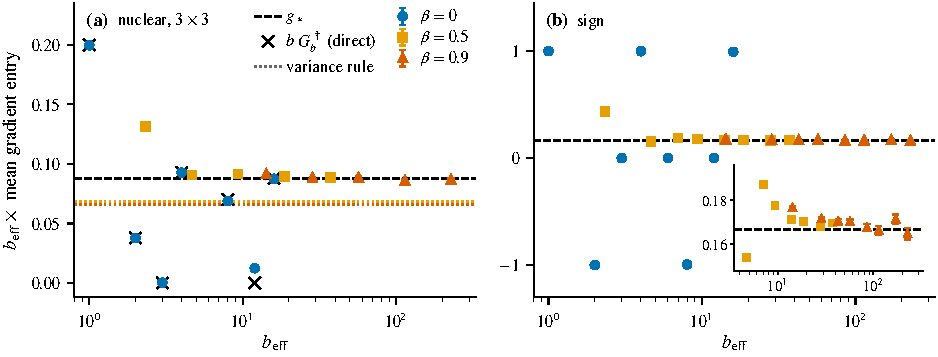
\includegraphics[width=\textwidth]{fig_momentum_discrete.pdf}
\caption{The stochastic iteration with momentum and lattice noise: $\beff$ times the mean entry of the limiting gradient,
against $\beff=b(1+\beta+\beta^2)/(1-\beta^2)$, for $b\in\{1,2,4,8,16\}$ and three values of $\beta$. (a) Orthogonalized
steps on $3\times3$ matrices; dashed: $\gs$; dotted: the value that the variance-effective batch size would give;
crosses: direct minimization for $\beta=0$. (b) Sign descent; inset: $\beta>0$.}
\label{fig:mom}
\end{figure}
\end{document}
